\documentclass[UTF8, a4paper, 11pt]{article}
\usepackage{diagbox}
\usepackage{subfigure}
\usepackage[UTF8, scheme=plain]{ctex}
\usepackage{fontspec}
\usepackage{float}
\usepackage{amsmath}
\newtheorem{myDef}{Definition}
\usepackage{graphicx}
\usepackage{geometry}
\usepackage{listings}
\usepackage{xcolor}
\usepackage{caption}
\geometry{scale=0.8}
\linespread{1.5}
\usepackage{hyperref}
\usepackage{color}
\usepackage{fontspec}
\usepackage{enumitem}
\usepackage[linesnumbered,boxed]{algorithm2e}    
\usepackage{xeCJK}
\usepackage{indentfirst} 
\graphicspath{{Pics/}} 	% 在于.tex同级的目录下创建名为pic的文件夹,存放图片


\setlength{\parindent}{2em}

\lstset{
    language={python},
    frame=shadowbox,
    breaklines=true,
    numbers=left,
    backgroundcolor=\color[RGB]{245,245,244},
    rulesepcolor=\color{red!20!green!20!blue!20},
    numberstyle={\color[RGB]{0,192,192}\tiny},
    basicstyle=\footnotesize \fontspec{Source Code Pro}
}
\setenumerate[1]{itemsep=0pt,partopsep=0pt,parsep=\parskip,topsep=0pt}
\setitemize[1]{itemsep=0pt,partopsep=0pt,parsep=\parskip,topsep=0pt}
\setdescription{itemsep=0pt,partopsep=0pt,parsep=\parskip,topsep=0pt}


\title{	
\normalfont \normalsize
\textsc{School of Data and Computer Science, Sun Yat-sen University} \\ [25pt] %textsc small capital letters
\rule{\textwidth}{0.5pt} \\[0.4cm] % Thin top horizontal rule
\huge 数电实验7\\ % The assignment title
\rule{\textwidth}{2pt} \\[0.5cm] % Thick bottom horizontal rule
\author{18308045 谷正阳}
\date{\normalsize\today}
}

\begin{document}
\maketitle
\tableofcontents
\newpage
\section{仿真实验}
\subsection{表决器}
\subsubsection{电路图}
用一位加法器实现,SW3拥有一票否决权。
\begin{figure}[H]
    \centering
    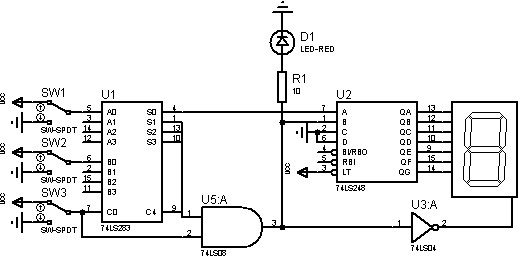
\includegraphics[width=0.8\textwidth]{ex7.1电路图.jpg}
\end{figure}
\subsubsection{静态实验结果}
\begin{figure}[H]
    \centering
    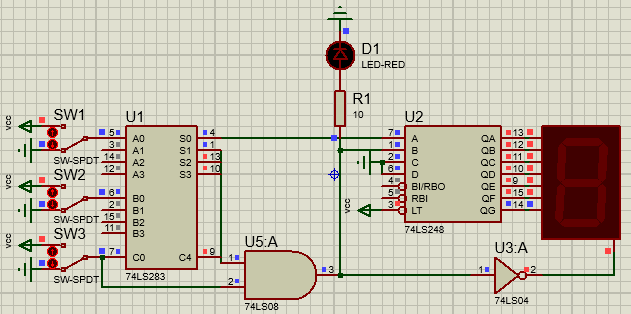
\includegraphics[width=0.8\textwidth]{000.png}
\end{figure}
\begin{figure}[H]
    \centering
    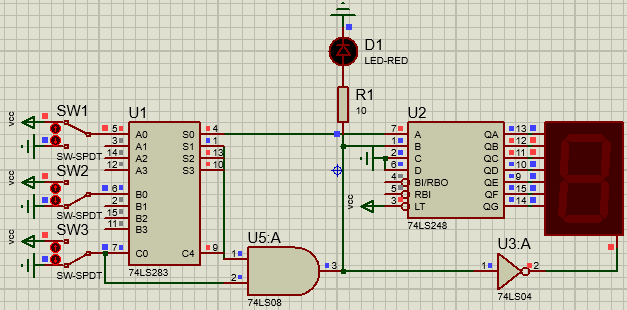
\includegraphics[width=0.8\textwidth]{001.png}
\end{figure}
\begin{figure}[H]
    \centering
    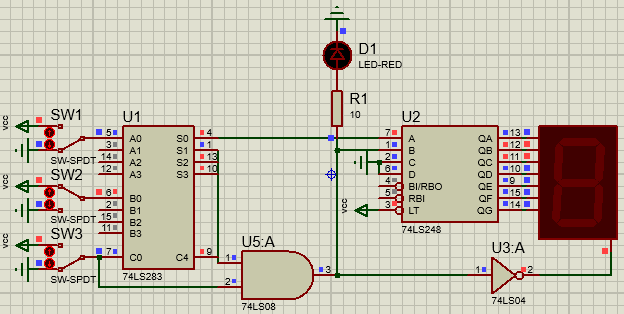
\includegraphics[width=0.8\textwidth]{010.png}
\end{figure}
\begin{figure}[H]
    \centering
    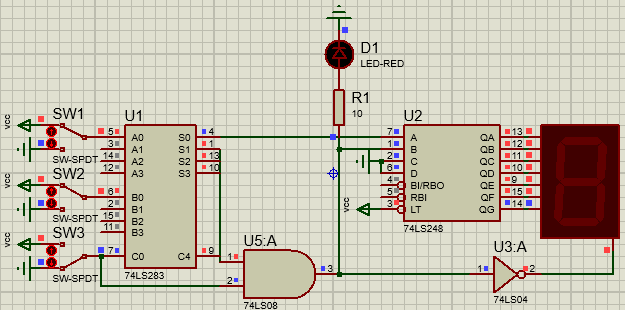
\includegraphics[width=0.8\textwidth]{011.png}
\end{figure}
\begin{figure}[H]
    \centering
    
\includegraphics[width=0.8\textwidth]{100.png}
\end{figure}
\begin{figure}[H]
    \centering
    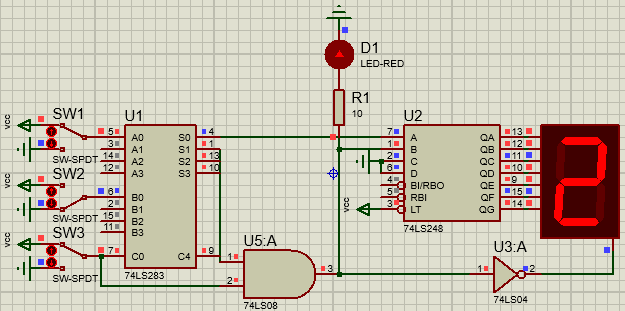
\includegraphics[width=0.8\textwidth]{101.png}
\end{figure}
\begin{figure}[H]
    \centering
    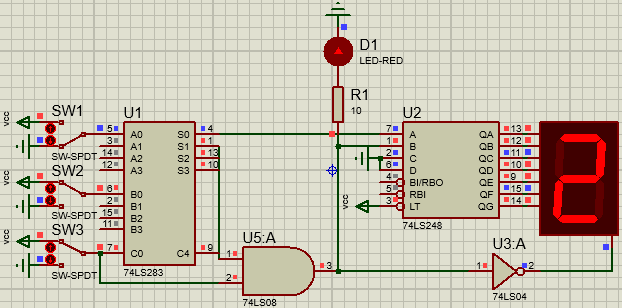
\includegraphics[width=0.8\textwidth]{110.png}
\end{figure}
\begin{figure}[H]
    \centering
    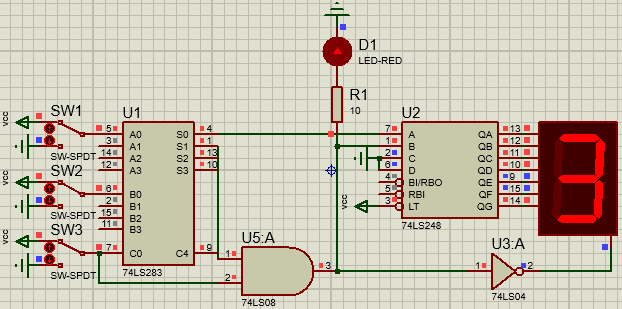
\includegraphics[width=0.8\textwidth]{111.png}
\end{figure}
\subsection{加法器}
\subsubsection{电路图}
SW1-4是A的低位到高位,SW5-8是B的低位到高位。S9是M,M=1是A-B。D1是CF,D2是OF。
\begin{figure}[H]
    \centering
    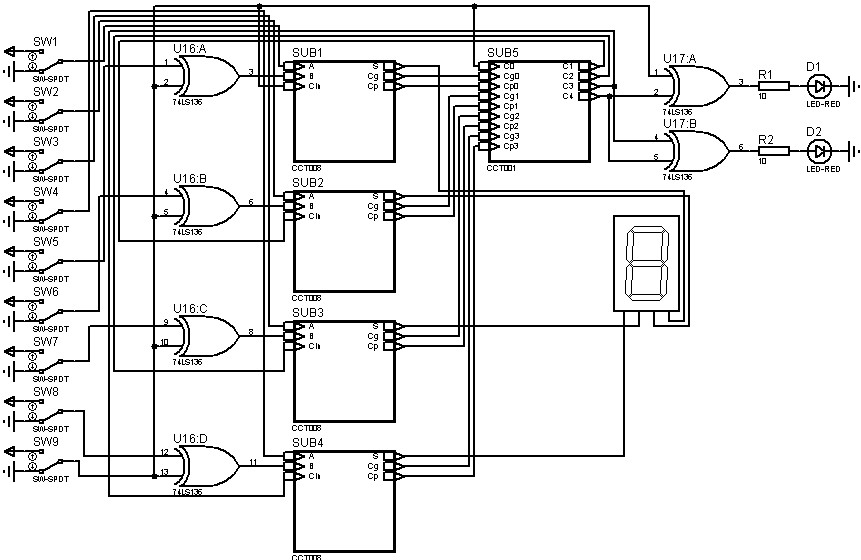
\includegraphics[width=0.8\textwidth]{ex7.2电路图.jpg}
\end{figure}
\subsubsection{静态实验设计}
用随机数生成SW1-9的取值:
\begin{lstlisting}
import random
random.seed(0)
[print([random.randint(0, 1) for _ in range(9)]) for _ in range(8)]
\end{lstlisting}
结果如下:
\begin{figure}[H]
    \centering
    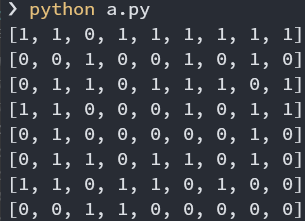
\includegraphics[width=0.8\textwidth]{rand.png}
\end{figure}
分别计算Y、CF、OF:
\begin{table}[H]
    \centering
\begin{tabular}{|l|l|l|l|l|l|}
\hline
A    & B    & M & Y    & CF & OF \\ \hline
1011 & 1111 & 1 & 1100 & 1  & 0  \\ \hline
0100 & 1010 & 0 & 1110 & 0  & 0  \\ \hline
0110 & 0111 & 1 & 1111 & 1  & 0  \\ \hline
0011 & 1010 & 1 & 1001 & 1  & 1  \\ \hline
0010 & 1000 & 0 & 1010 & 0  & 0  \\ \hline
0110 & 1011 & 0 & 0001 & 1  & 0  \\ \hline
1011 & 0101 & 0 & 0000 & 1  & 0  \\ \hline
1100 & 0000 & 0 & 1100 & 0  & 0  \\ \hline
\end{tabular}
\end{table}
\subsubsection{静态实验结果}
\begin{figure}[H]
    \centering
    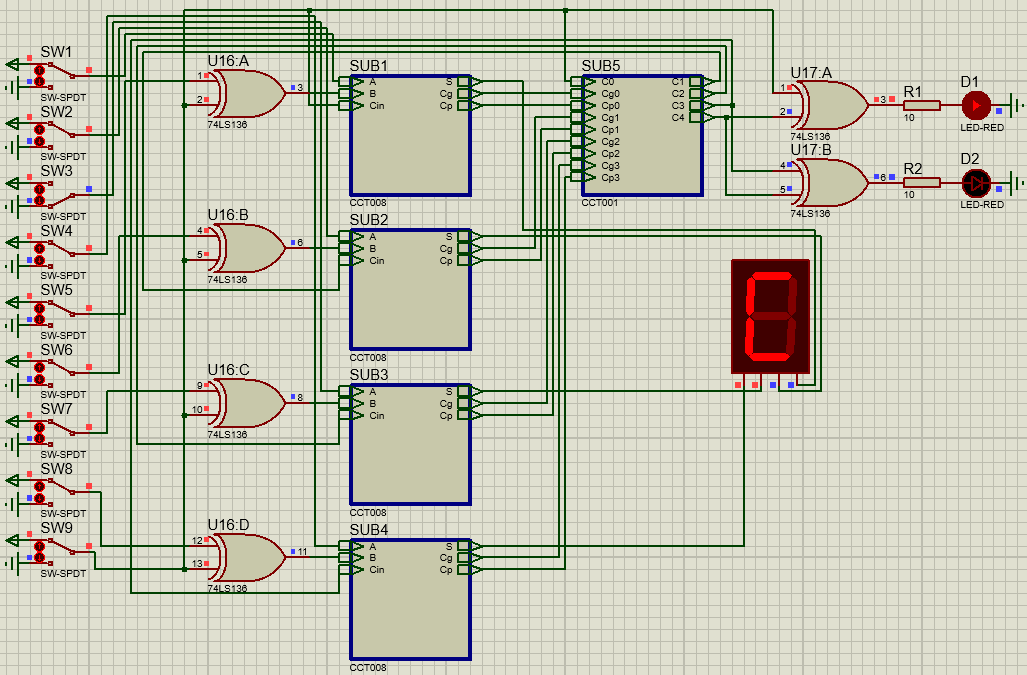
\includegraphics[width=0.8\textwidth]{1.png}
\end{figure}
\begin{figure}[H]
    \centering
    
\includegraphics[width=0.8\textwidth]{2.png}
\end{figure}
\begin{figure}[H]
    \centering
    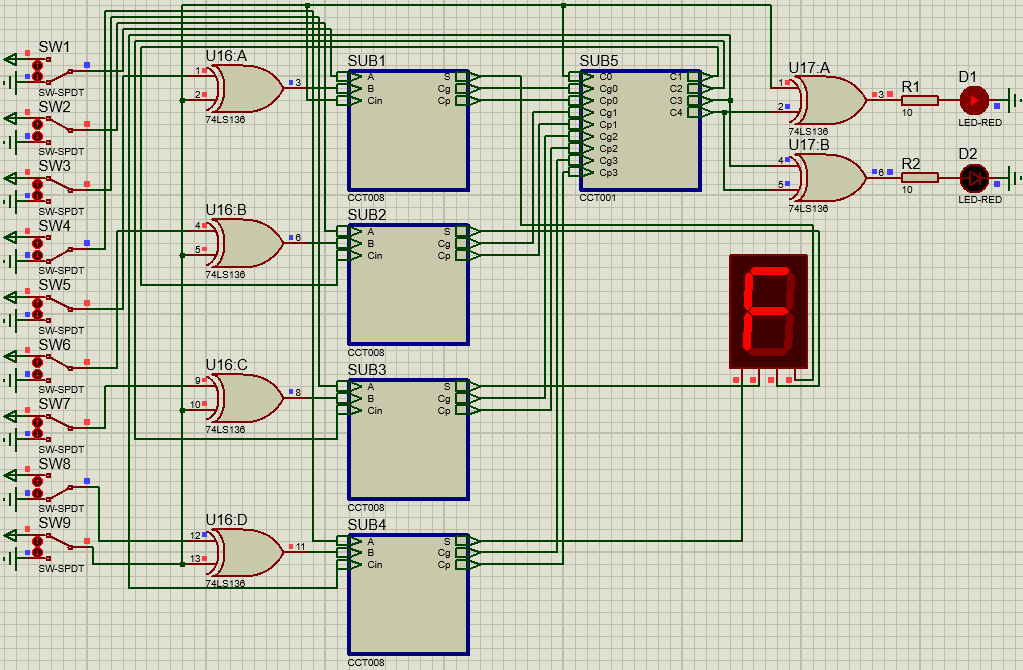
\includegraphics[width=0.8\textwidth]{3.png}
\end{figure}
\begin{figure}[H]
    \centering
    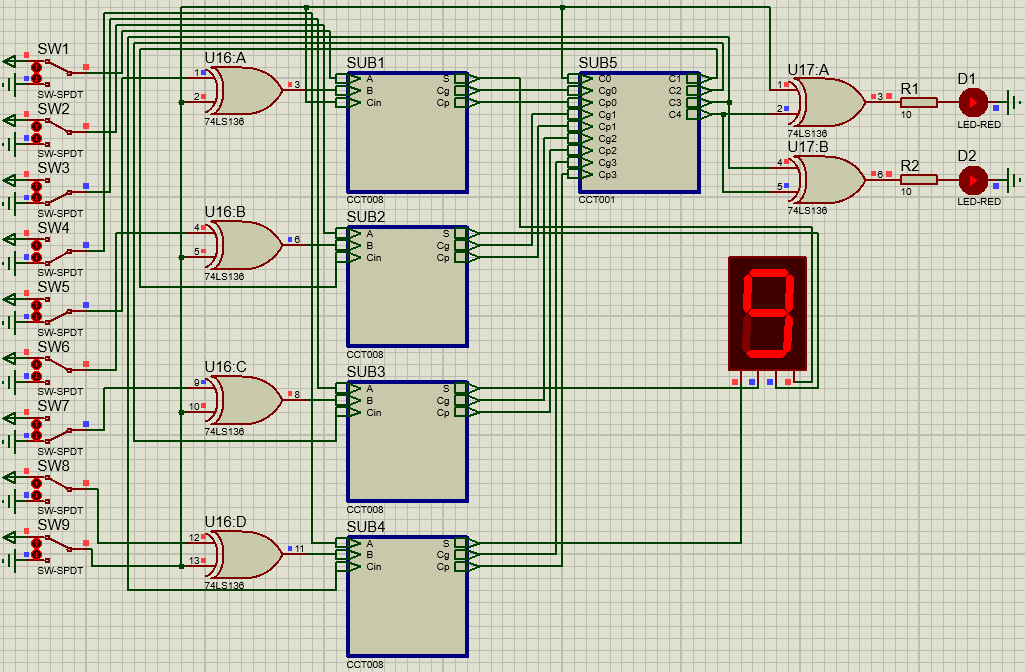
\includegraphics[width=0.8\textwidth]{4.png}
\end{figure}
\begin{figure}[H]
    \centering
    
\includegraphics[width=0.8\textwidth]{5.png}
\end{figure}
\begin{figure}[H]
    \centering
    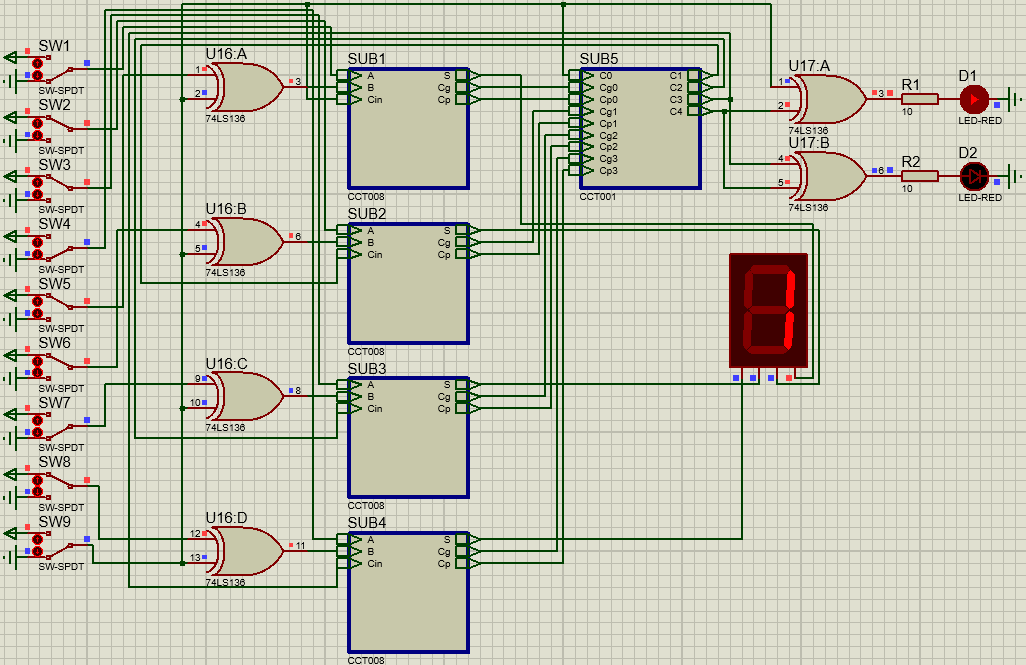
\includegraphics[width=0.8\textwidth]{6.png}
\end{figure}
\begin{figure}[H]
    \centering
    
\includegraphics[width=0.8\textwidth]{7.png}
\end{figure}
\begin{figure}[H]
    \centering
    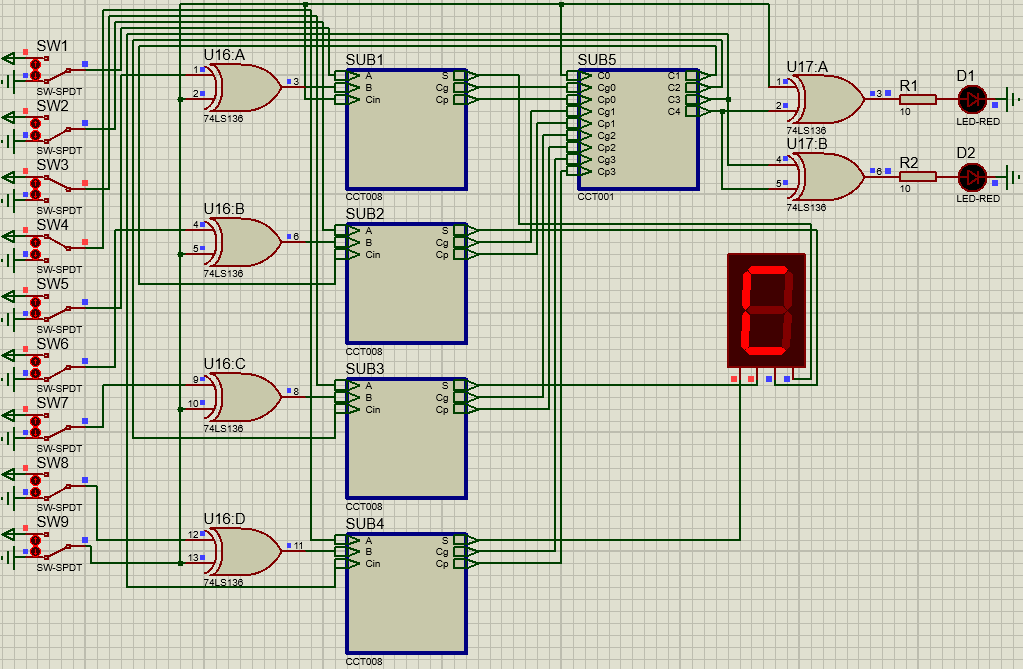
\includegraphics[width=0.8\textwidth]{8.png}
\end{figure}
\section{实验箱实验}
\subsection{表决器}
\begin{figure}[H]
    \centering
    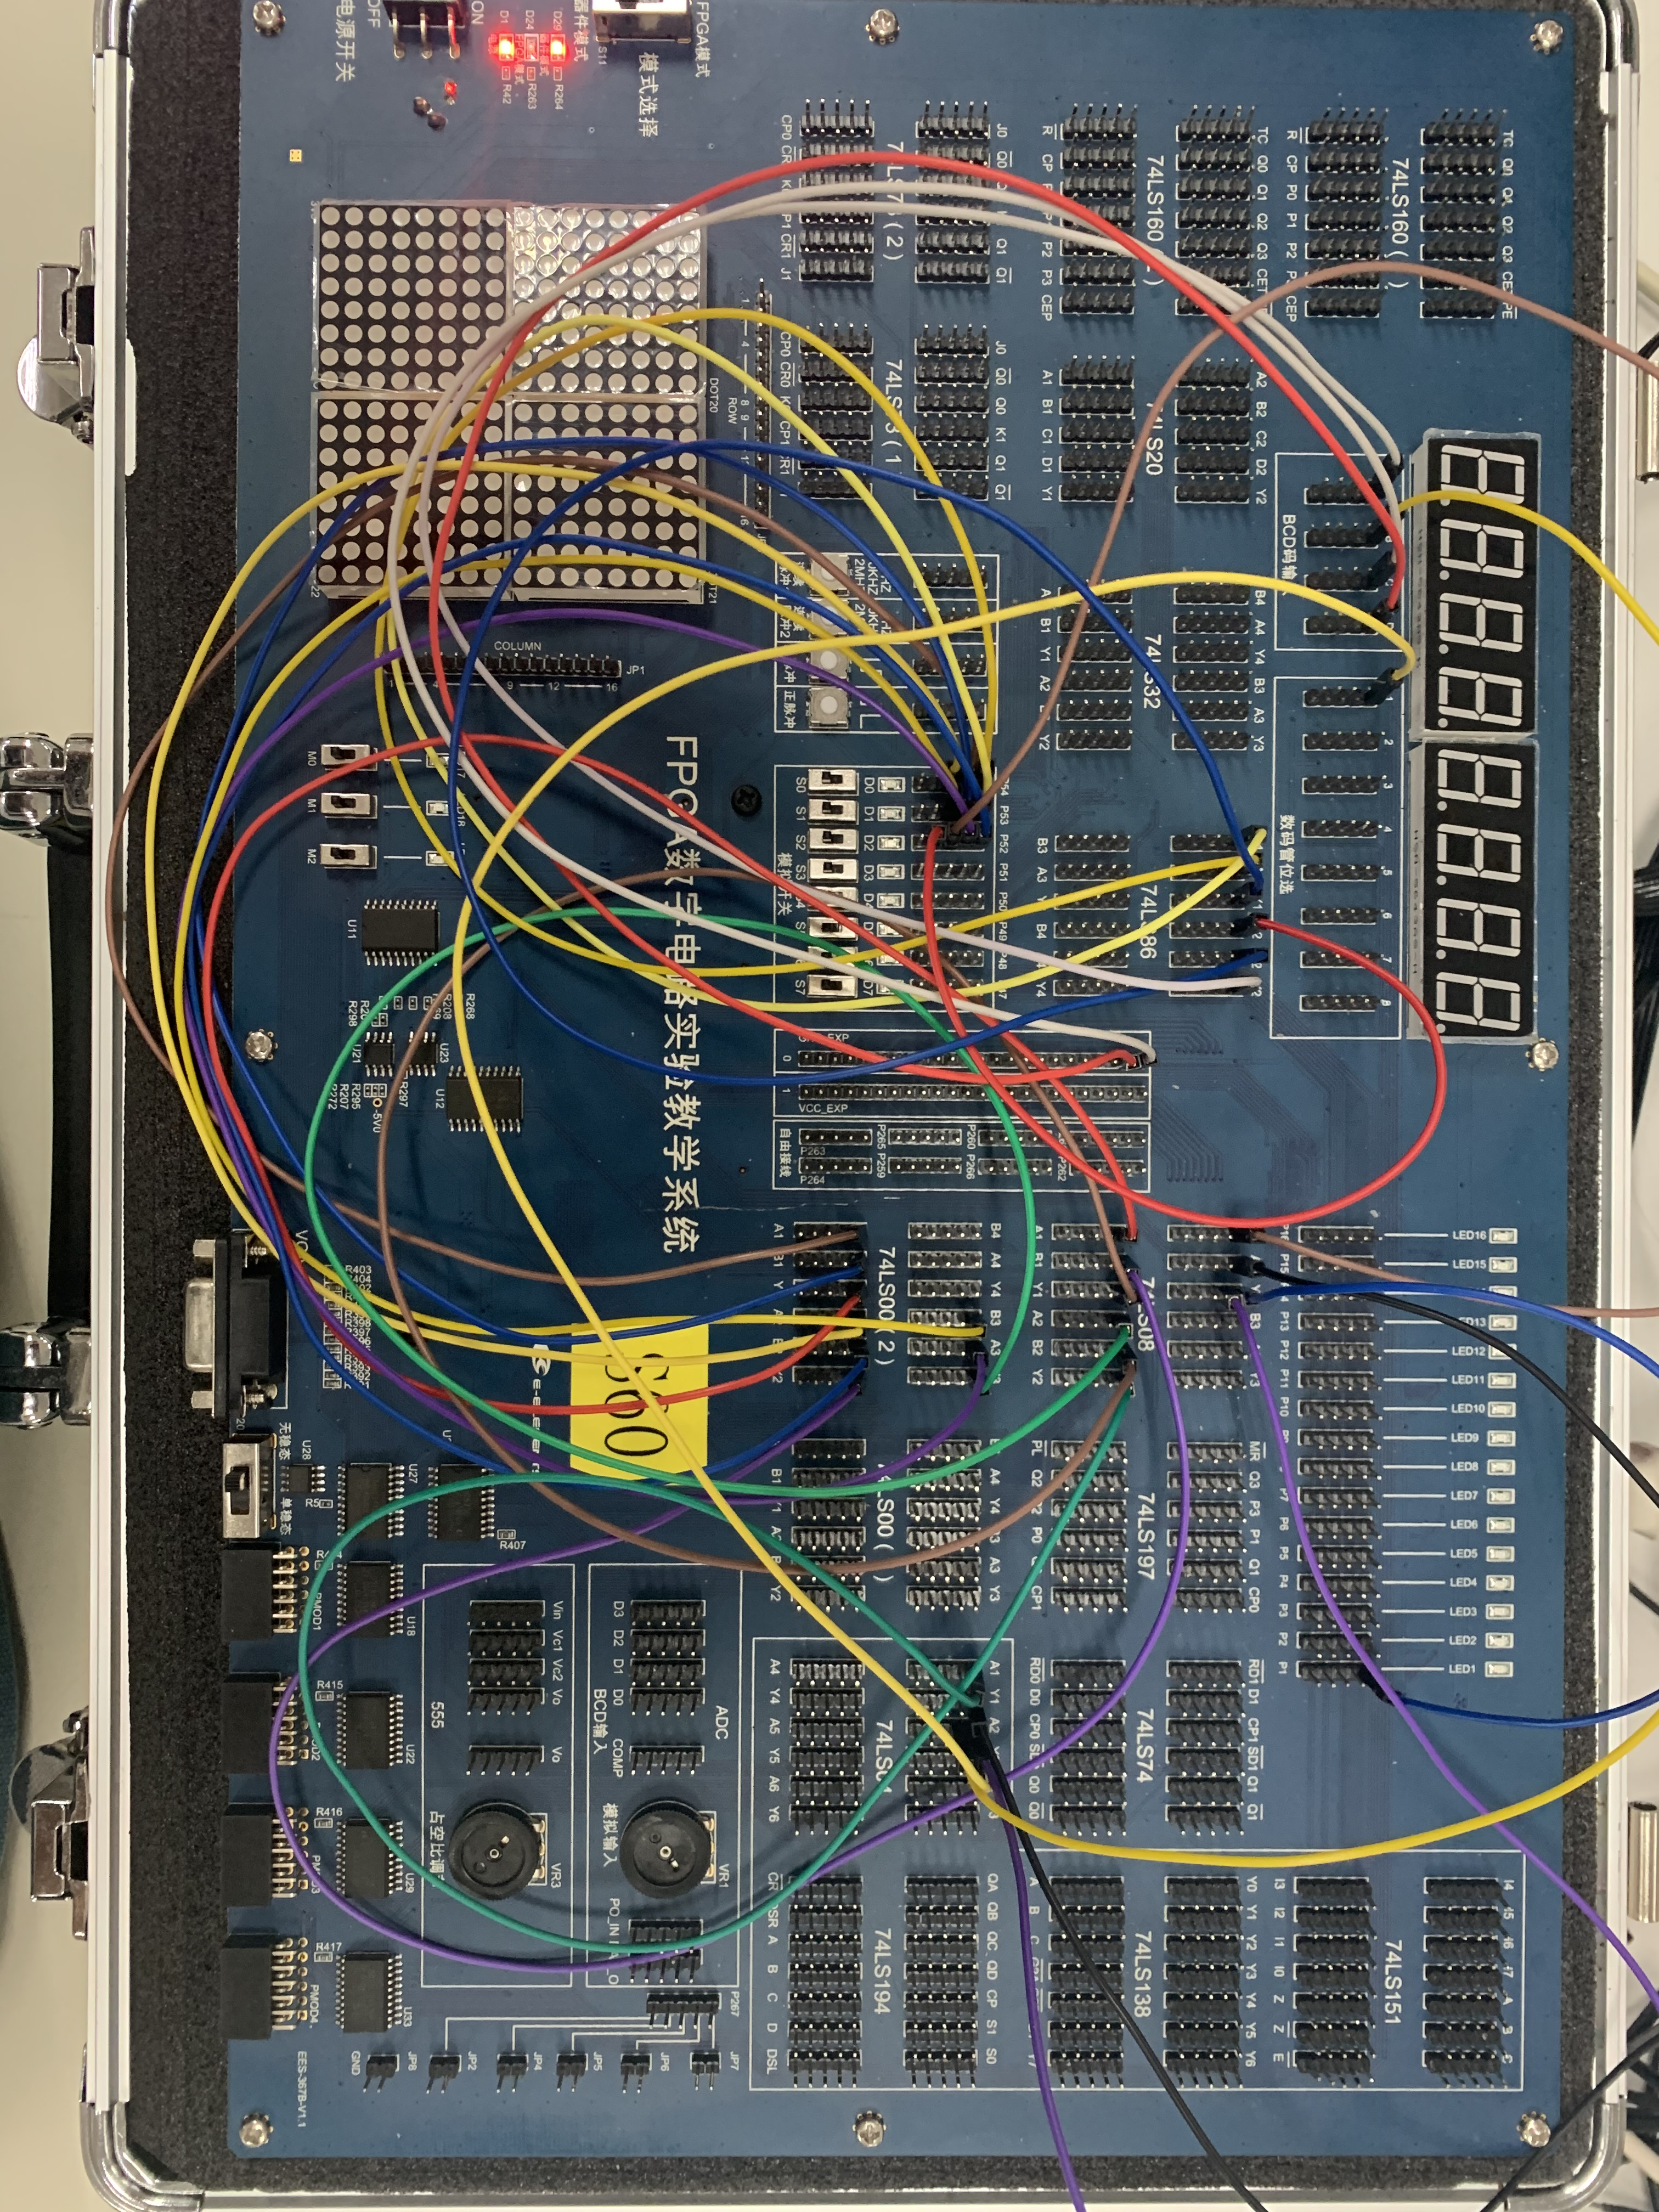
\includegraphics[width=0.8\textwidth]{箱000.png}
\end{figure}
\begin{figure}[H]
    \centering
    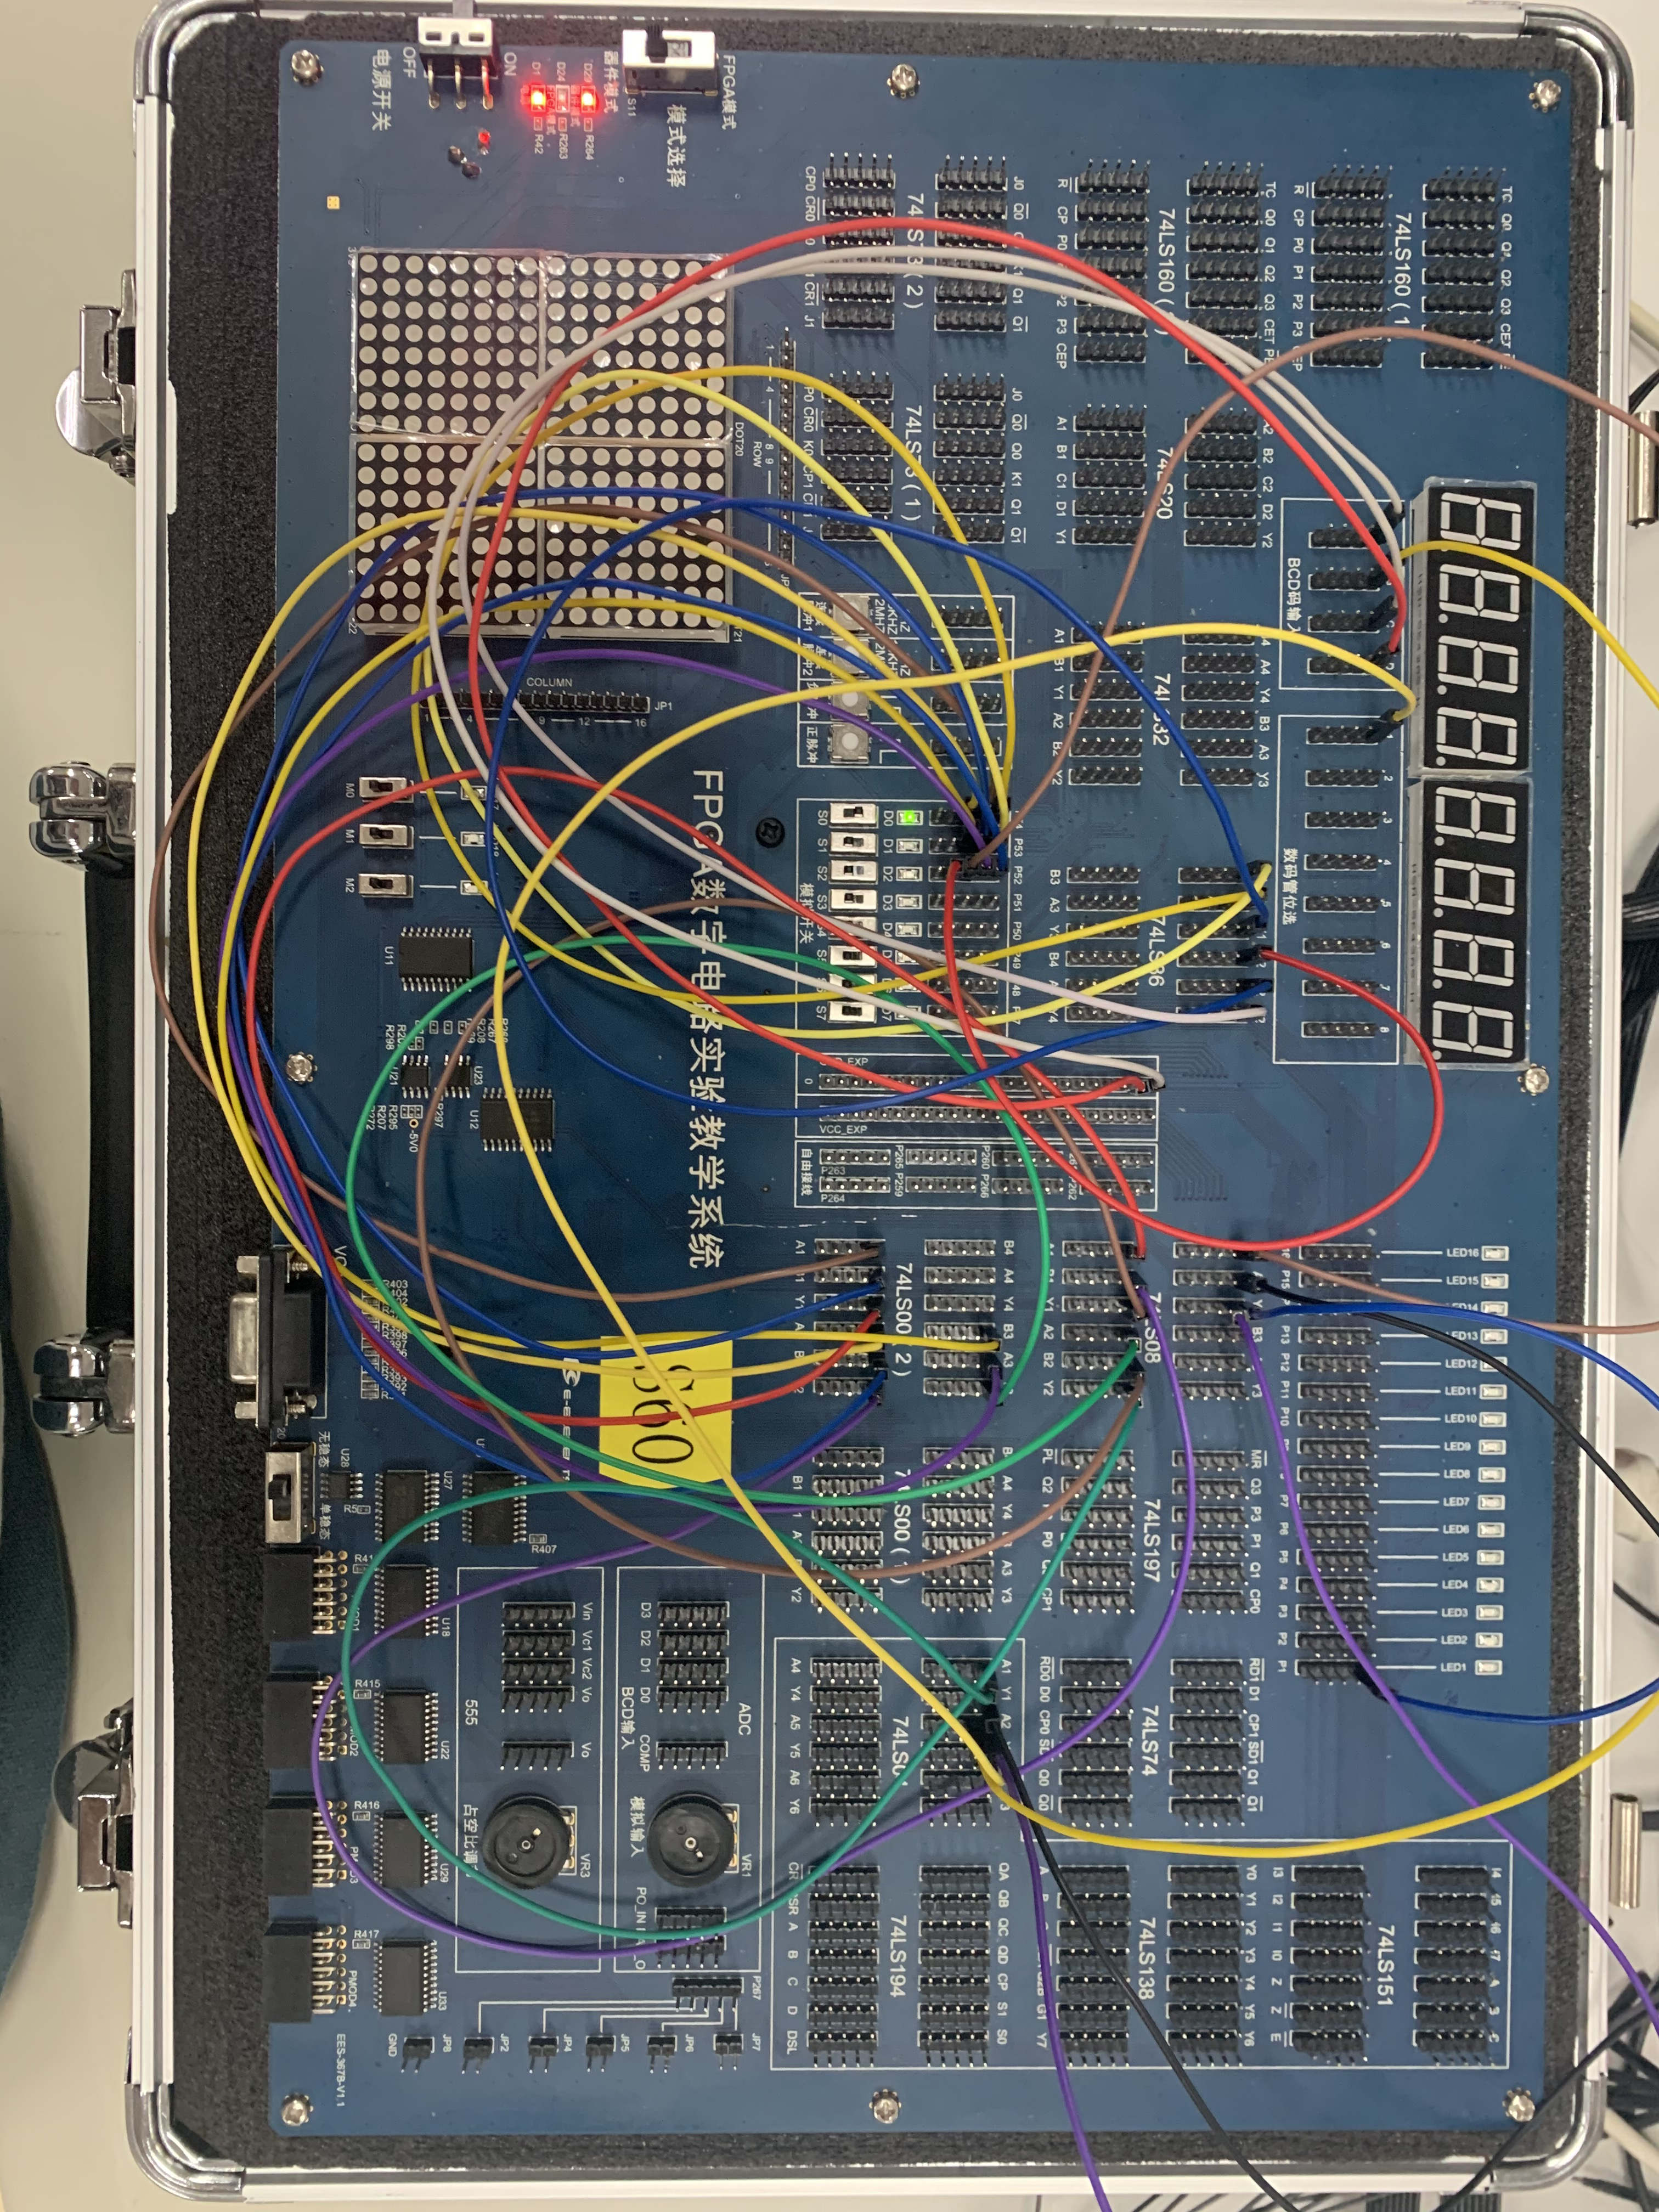
\includegraphics[width=0.8\textwidth]{箱001.png}
\end{figure}
\begin{figure}[H]
    \centering
    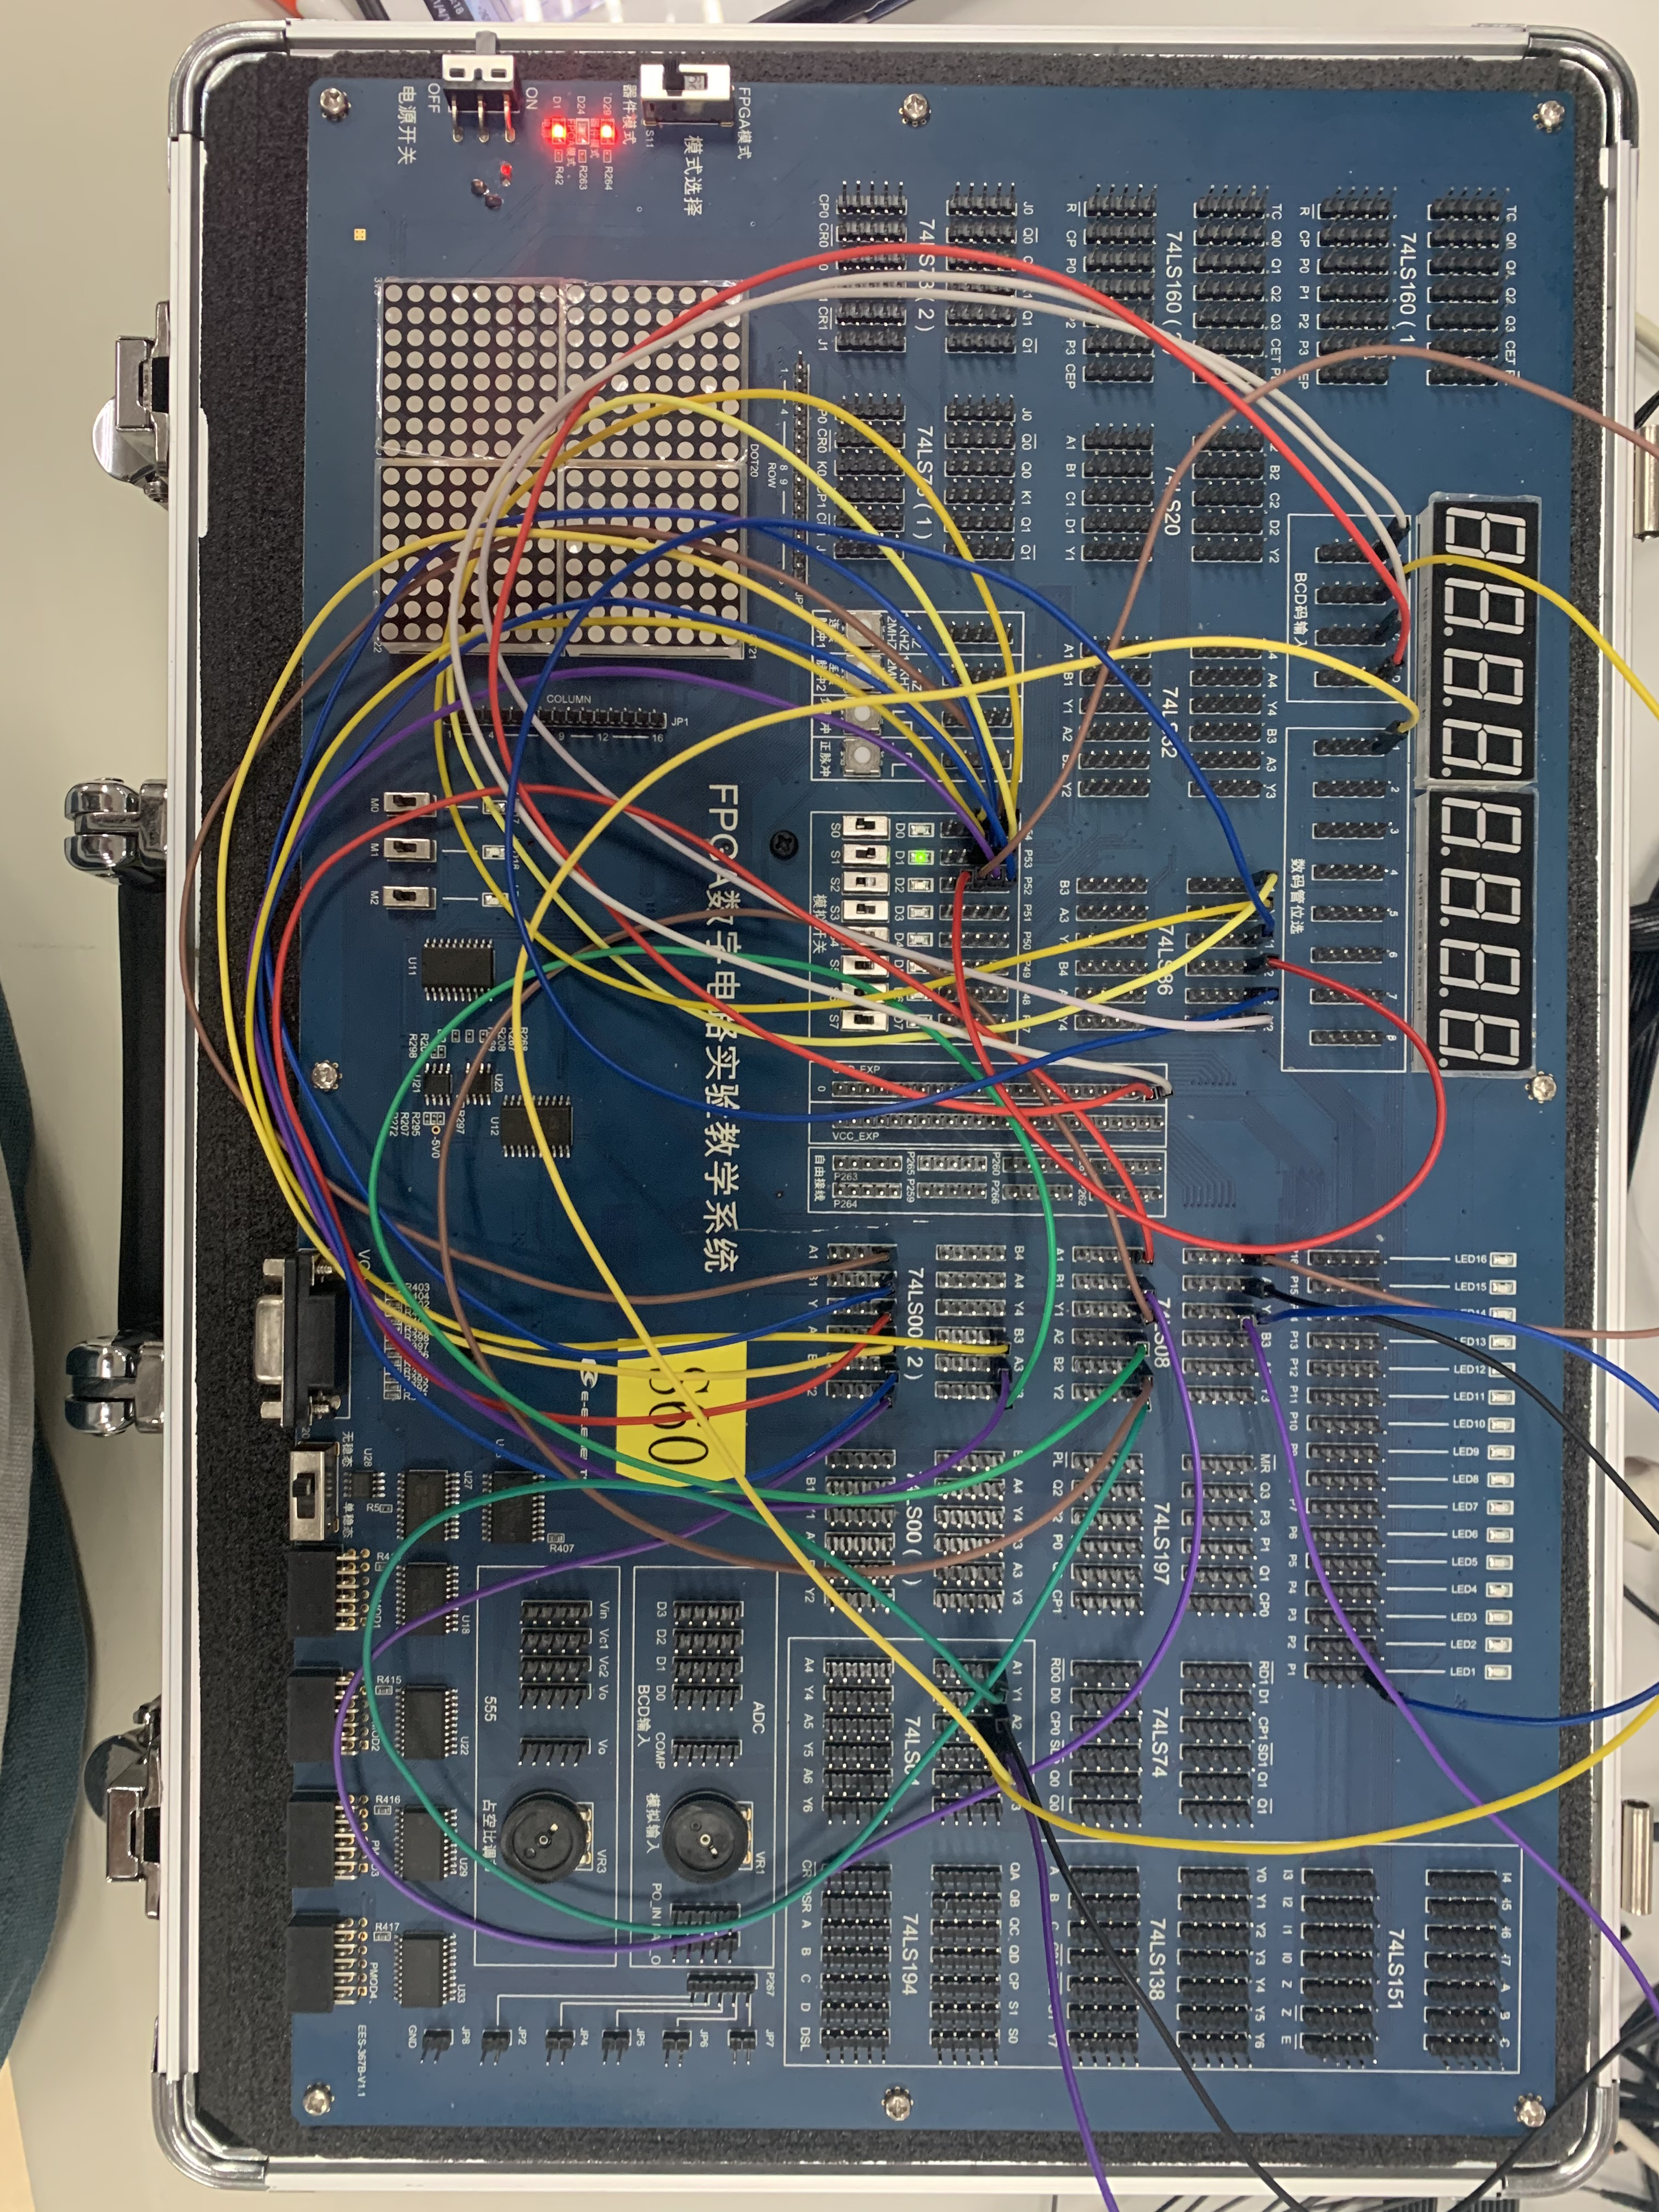
\includegraphics[width=0.8\textwidth]{箱010.png}
\end{figure}
\begin{figure}[H]
    \centering
    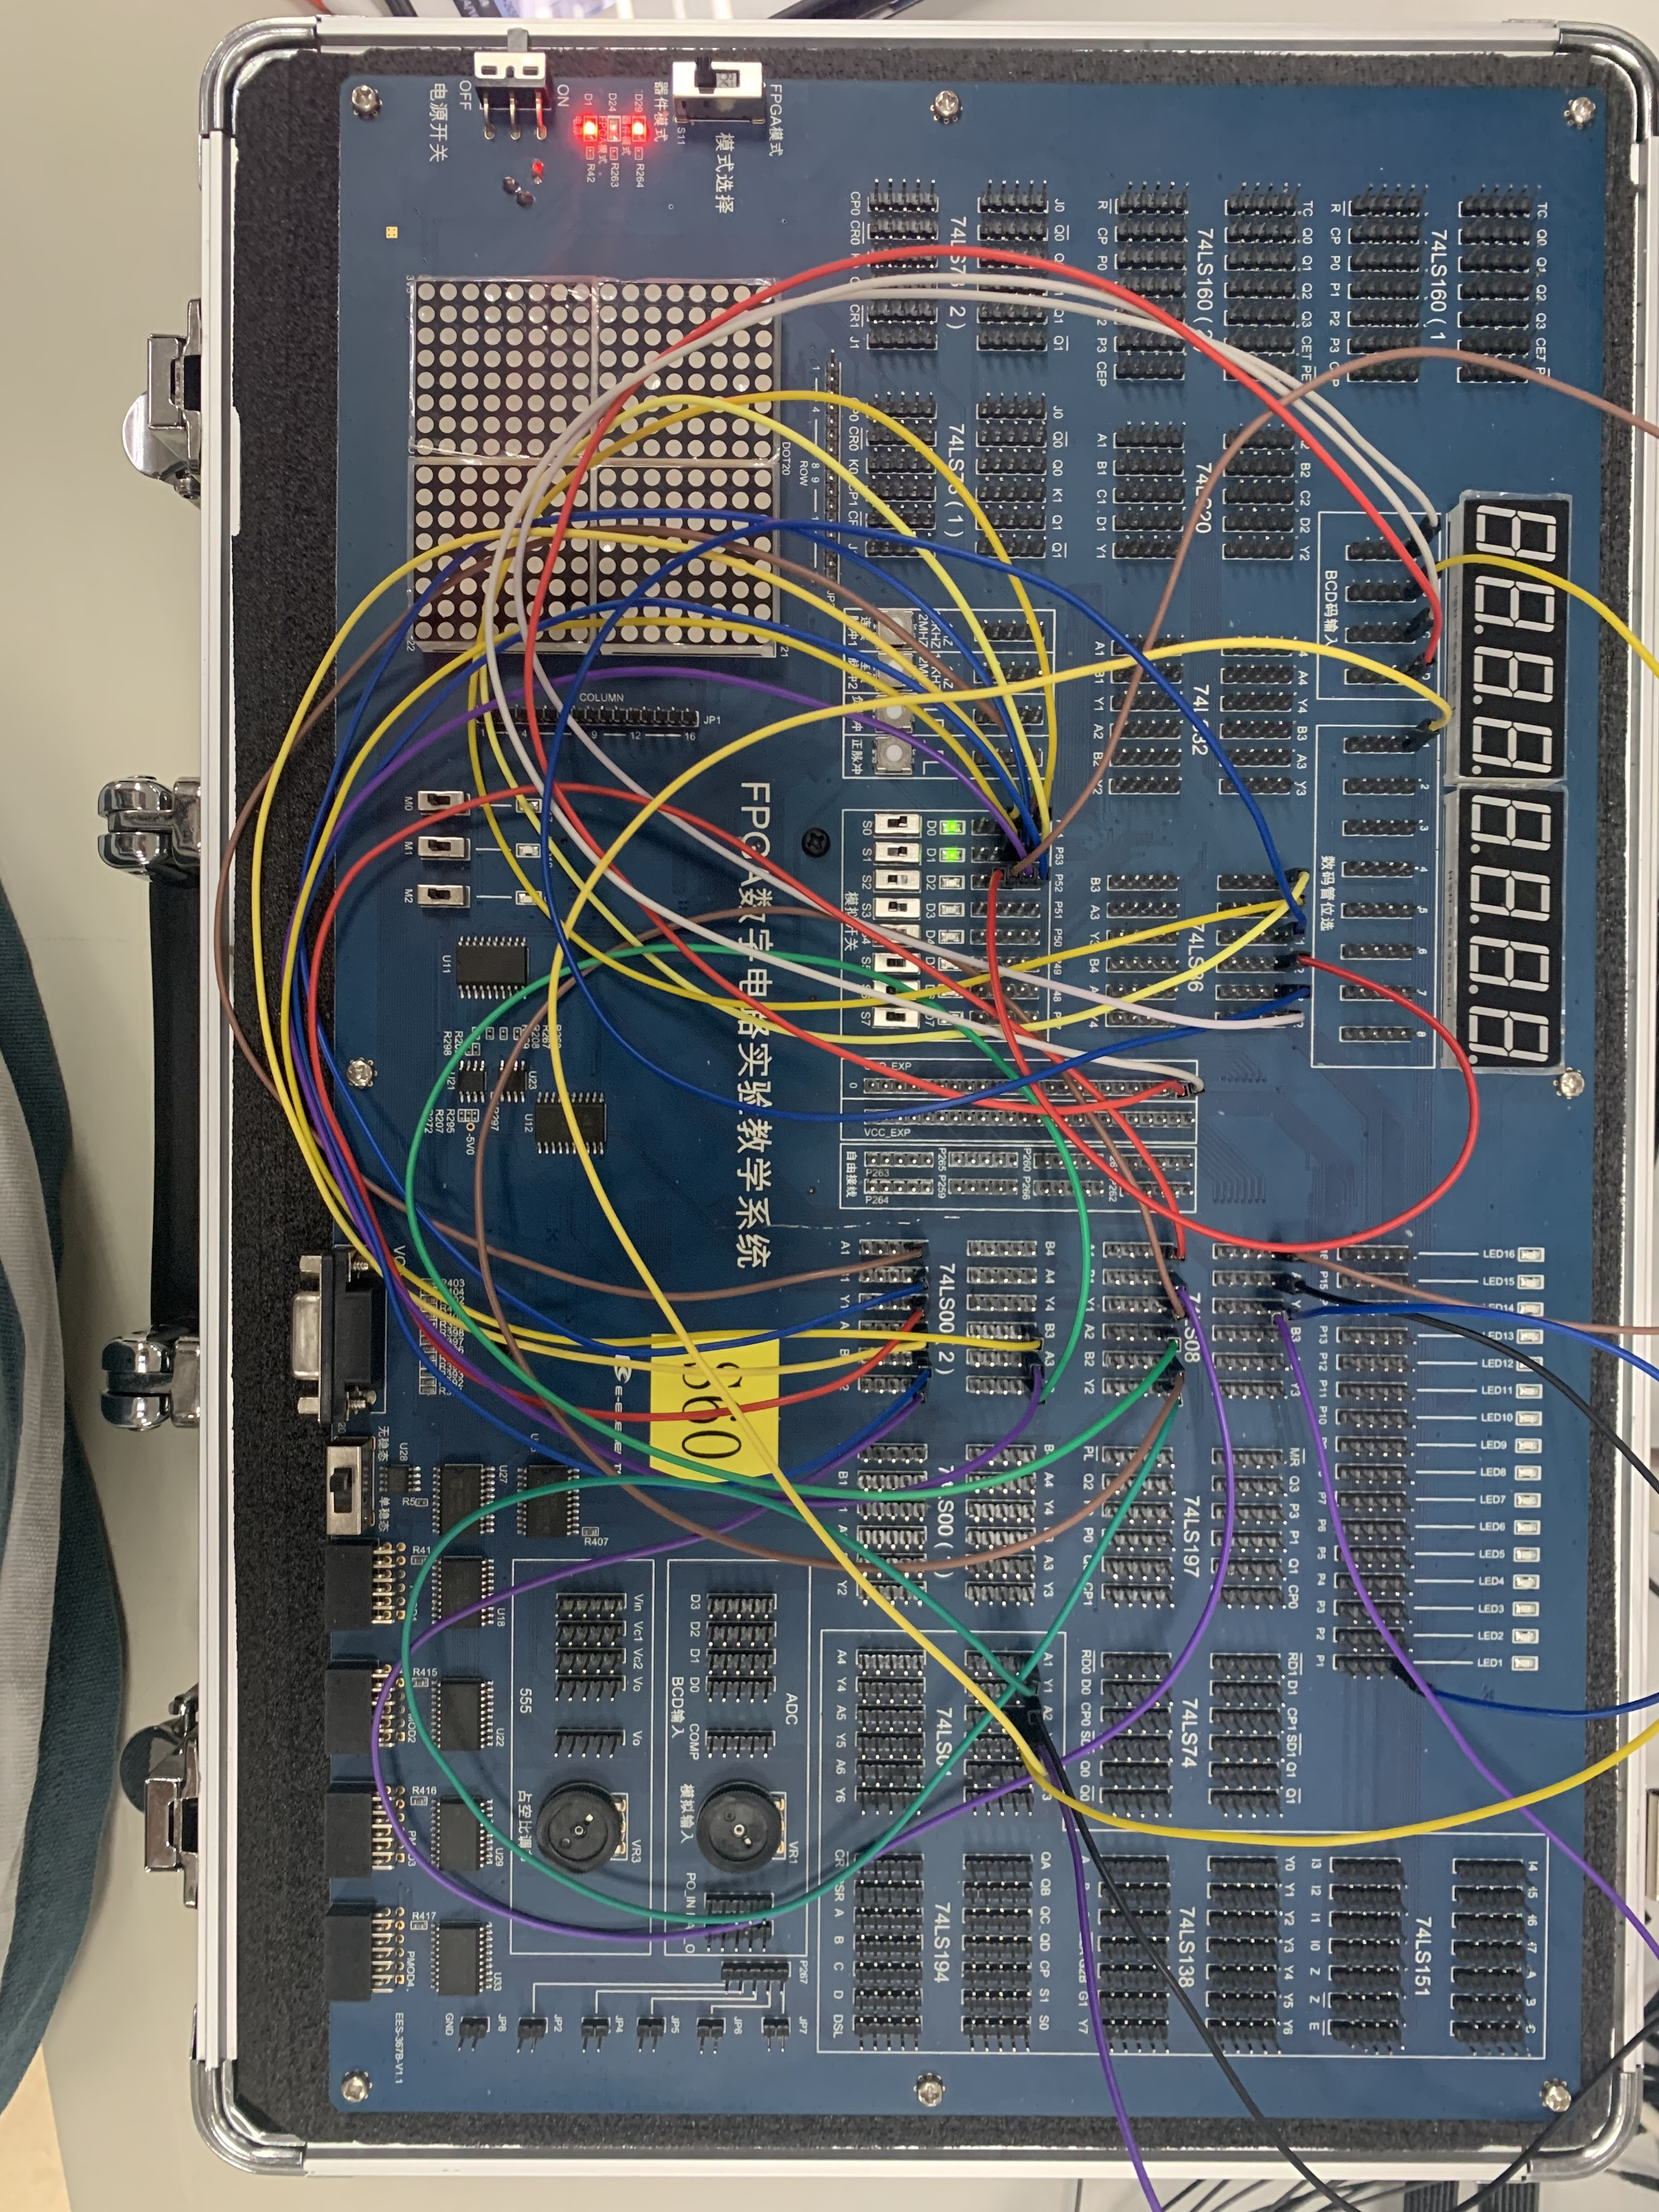
\includegraphics[width=0.8\textwidth]{箱011.png}
\end{figure}
\begin{figure}[H]
    \centering
    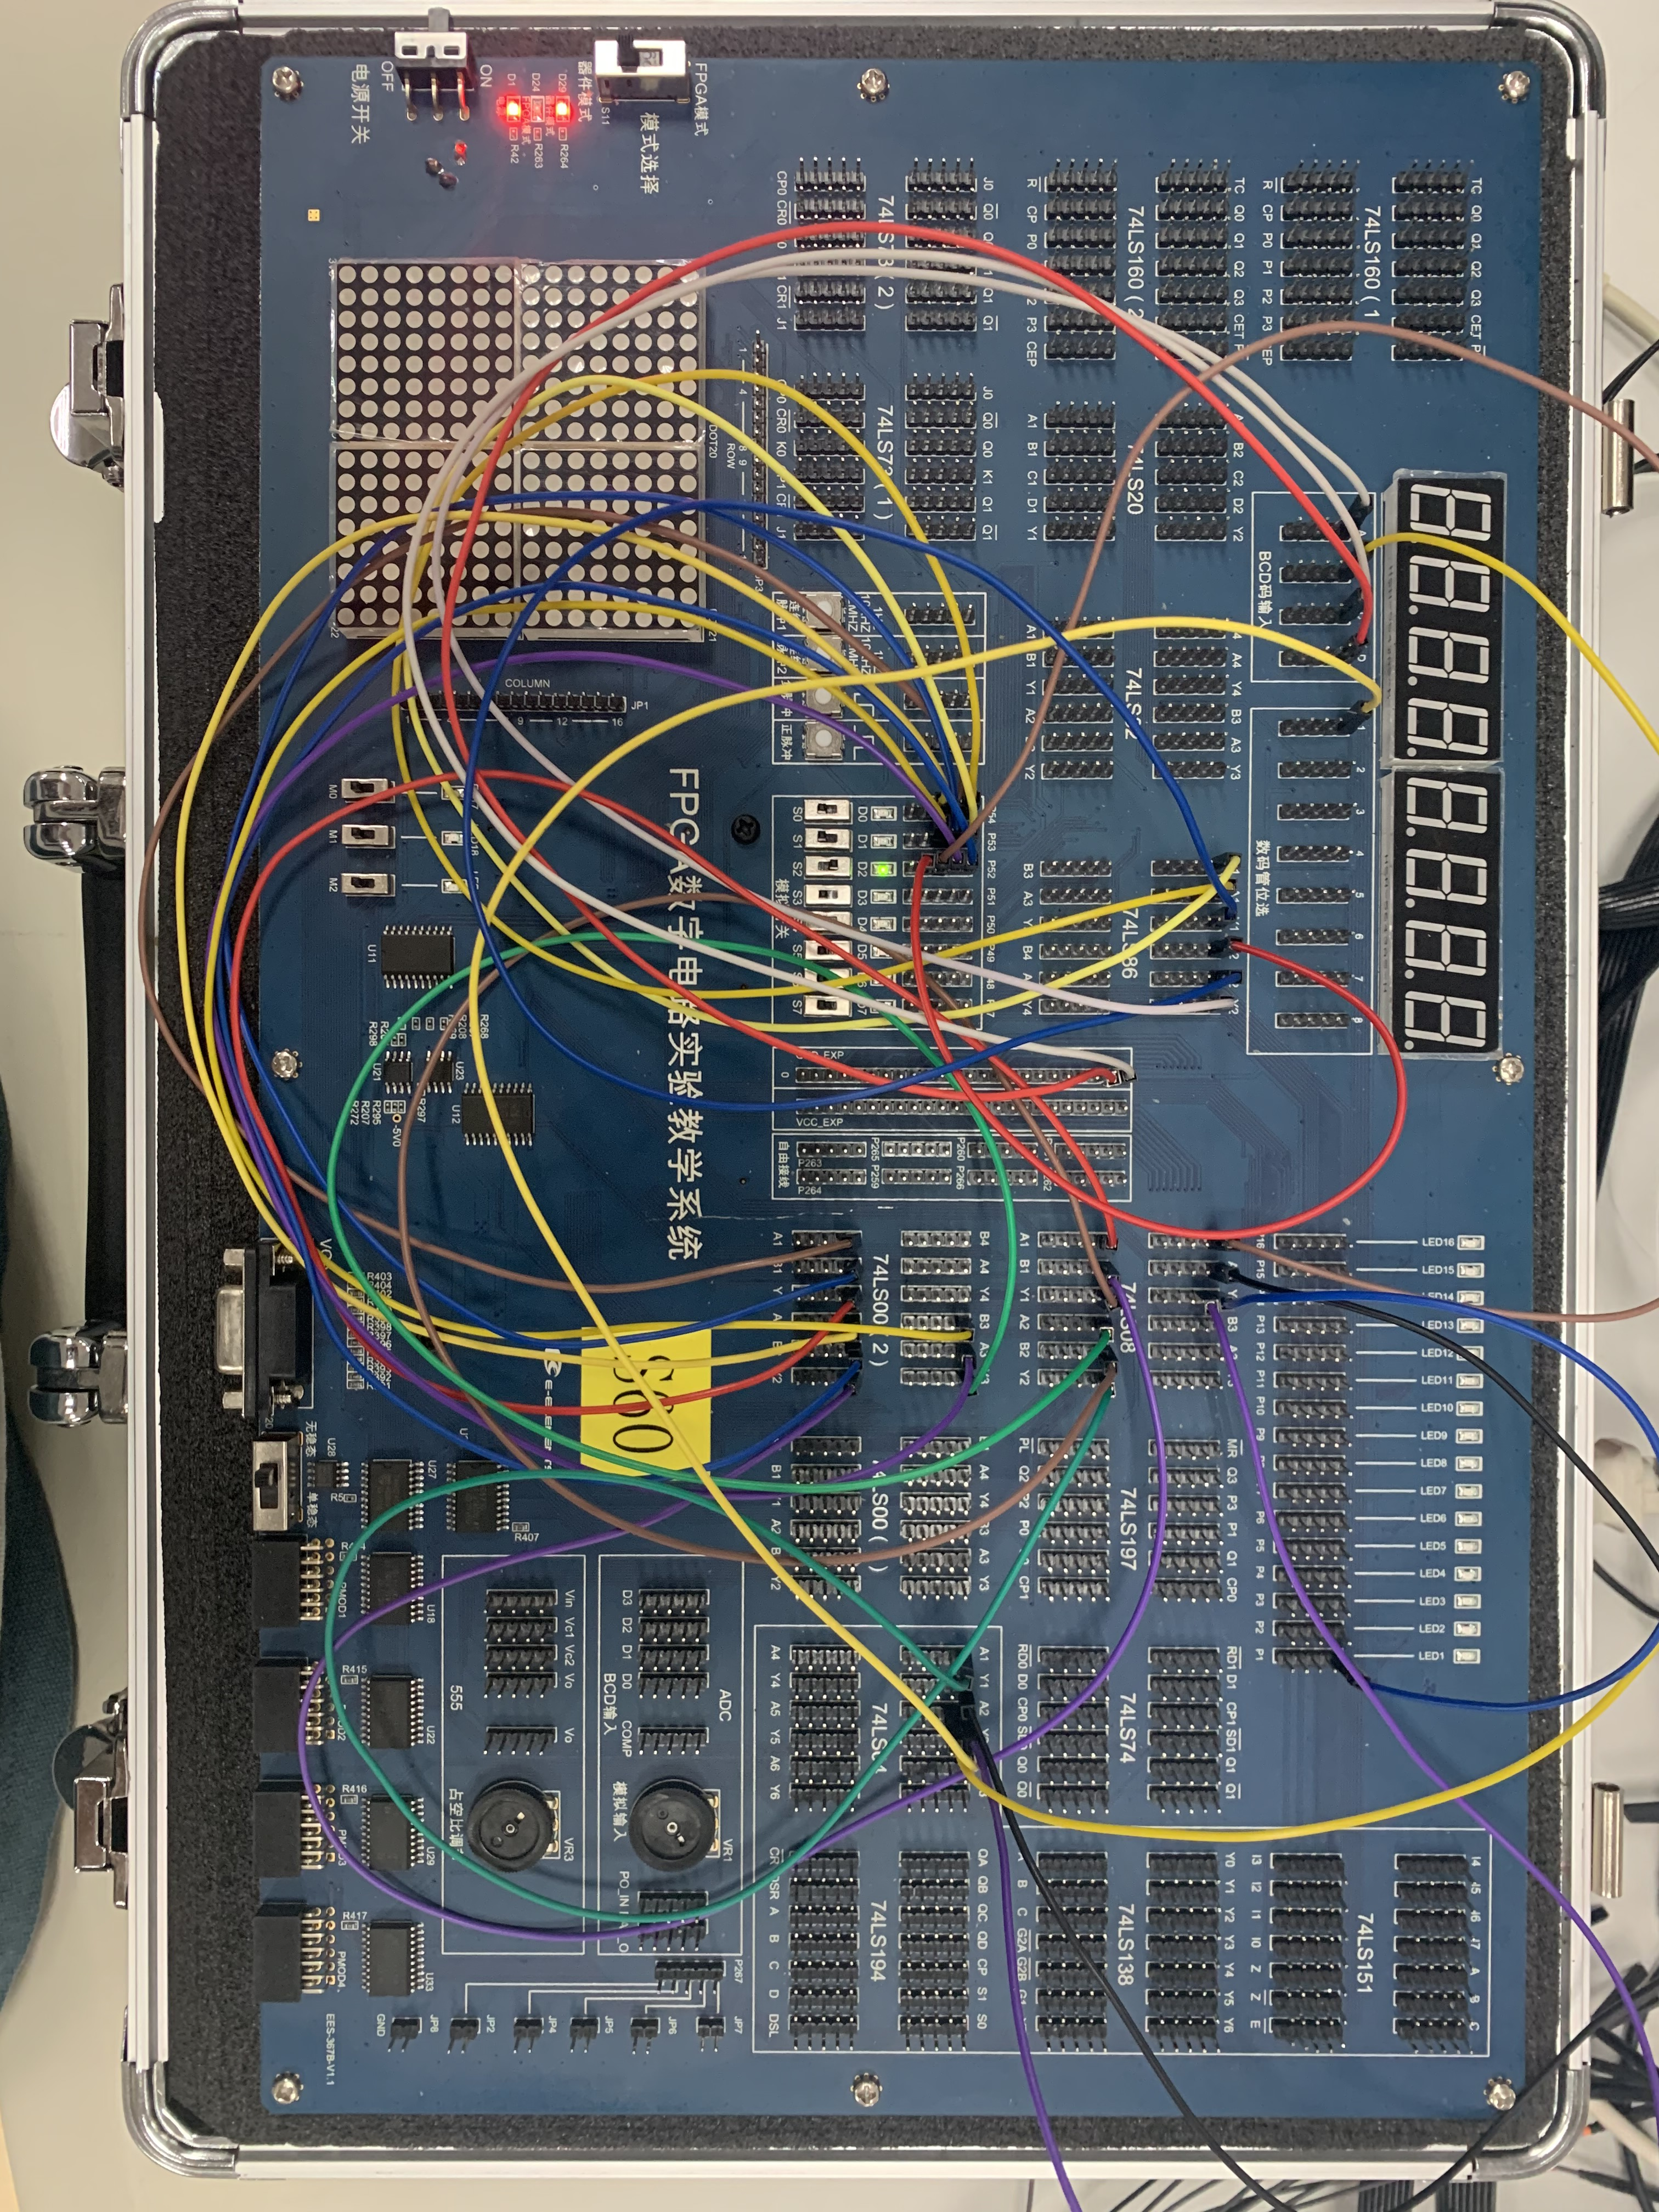
\includegraphics[width=0.8\textwidth]{箱100.png}
\end{figure}
\begin{figure}[H]
    \centering
    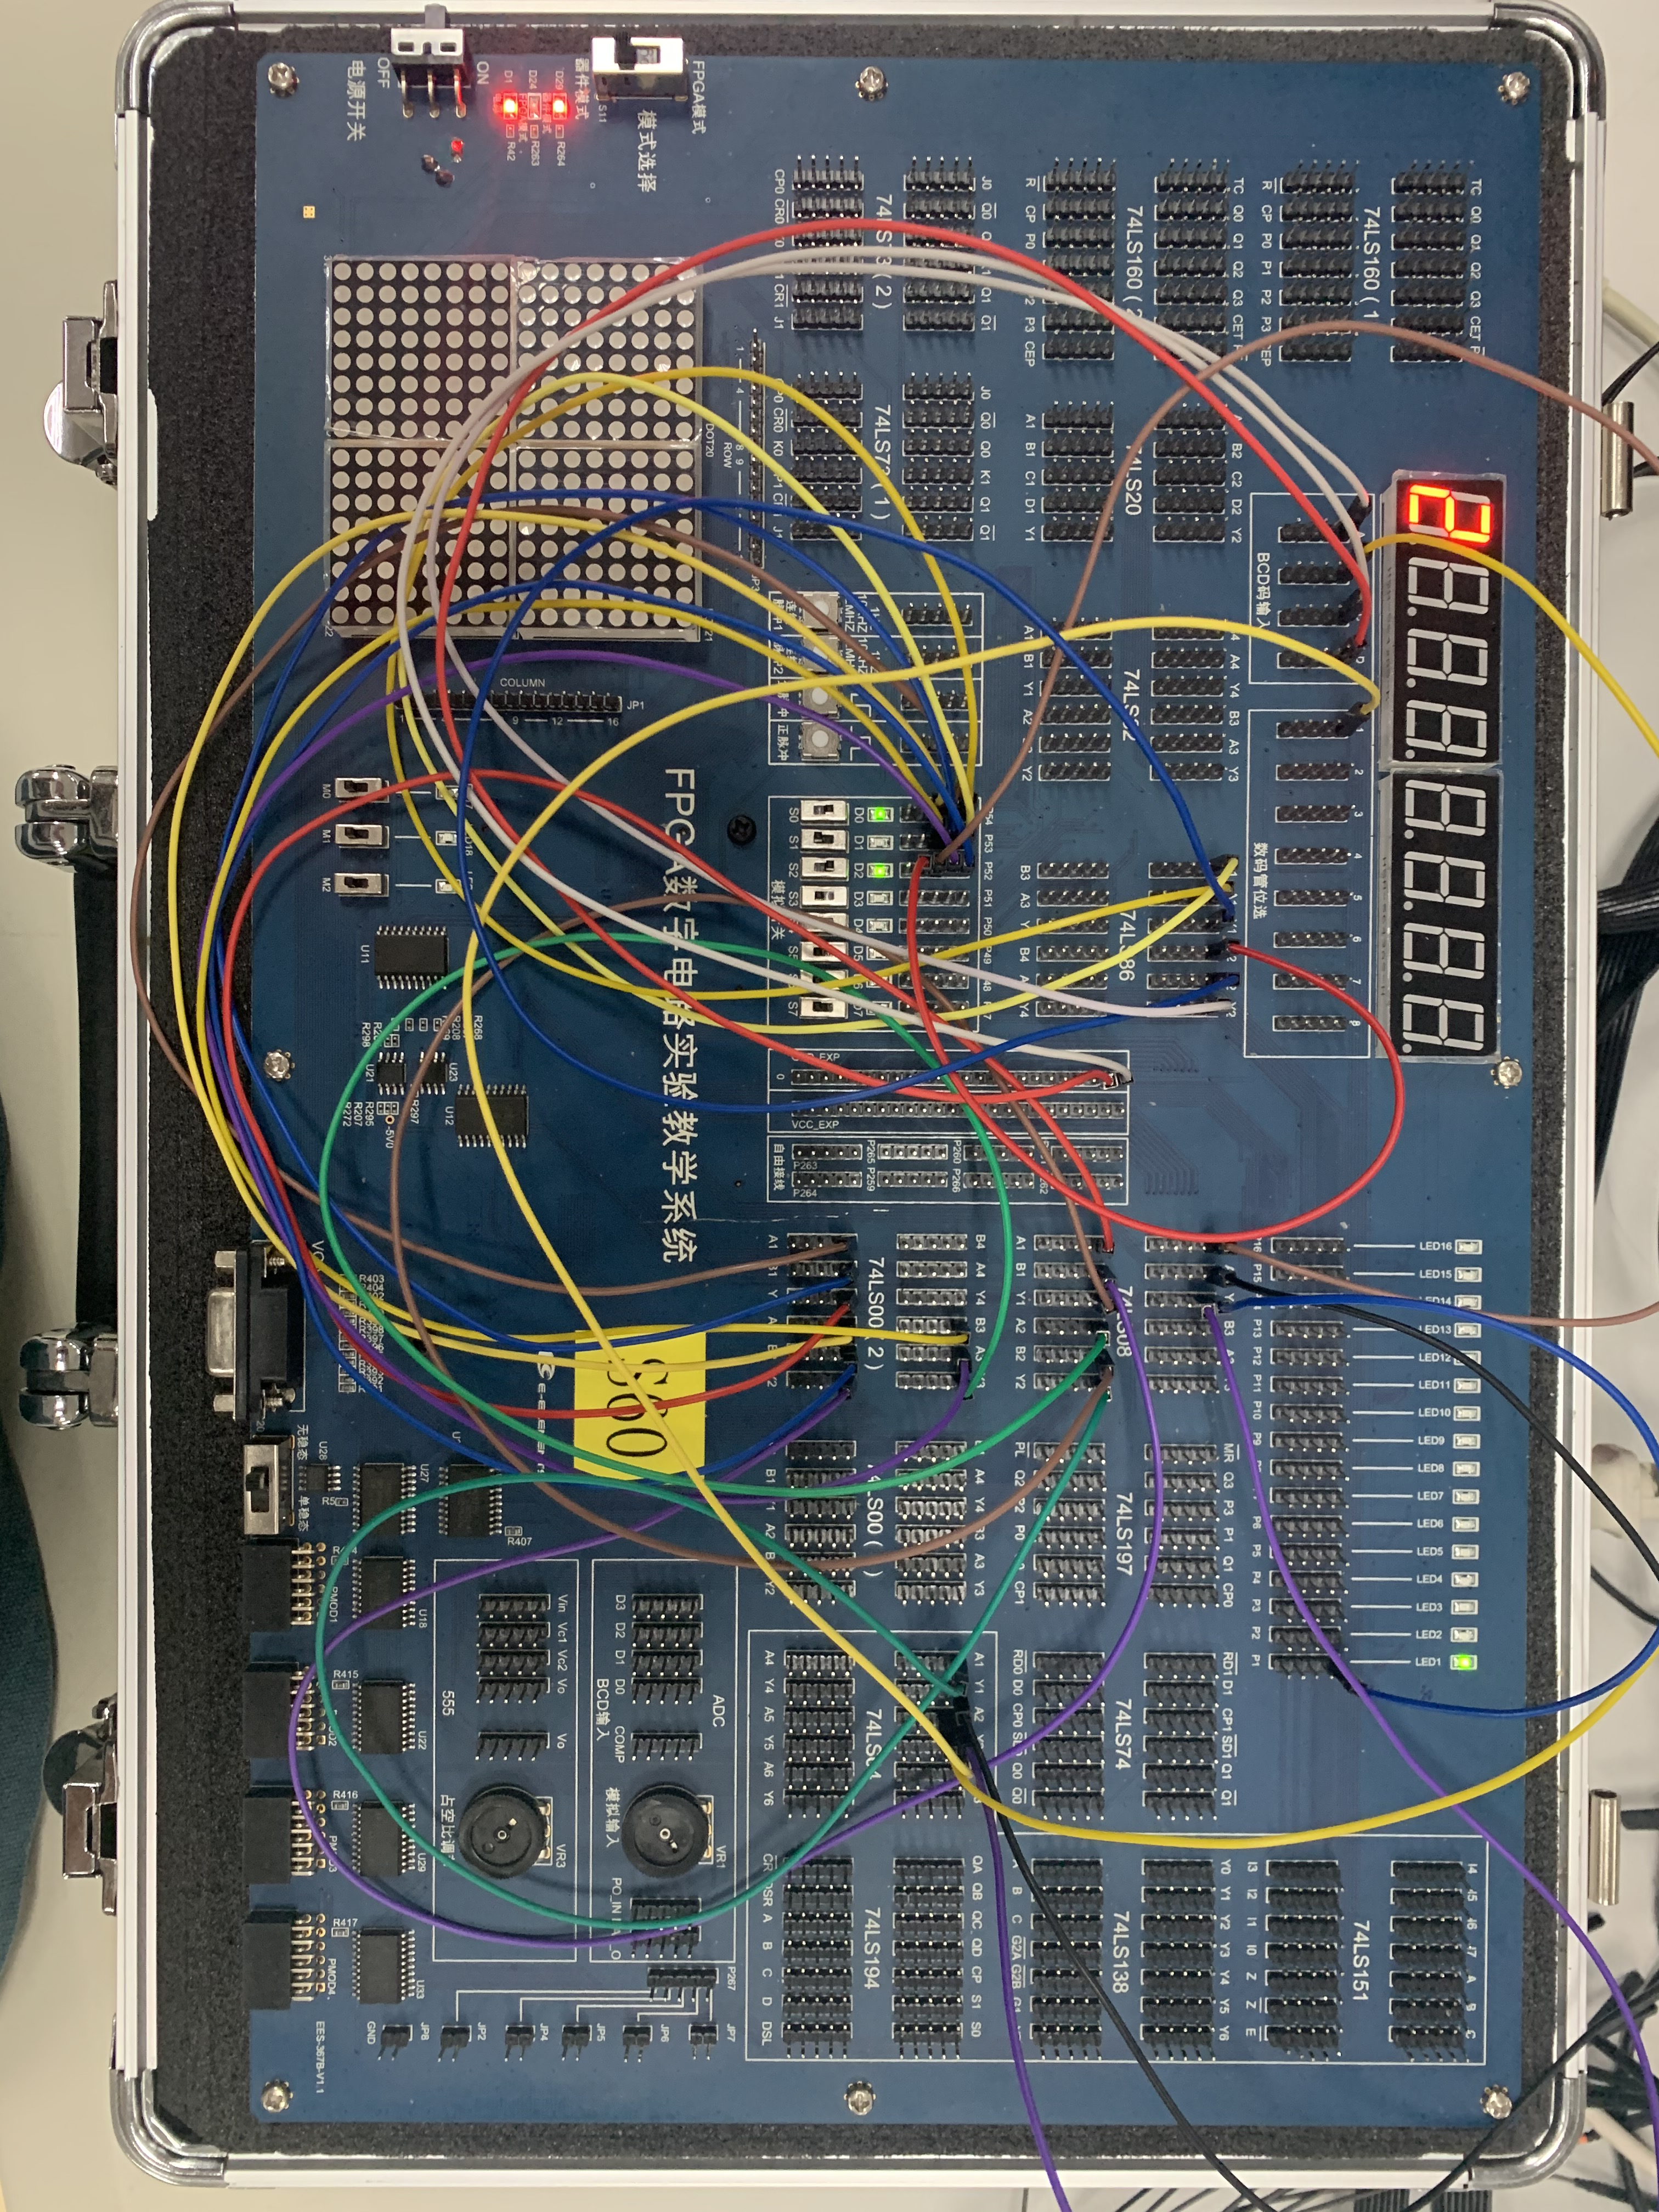
\includegraphics[width=0.8\textwidth]{箱101.png}
\end{figure}
\begin{figure}[H]
    \centering
    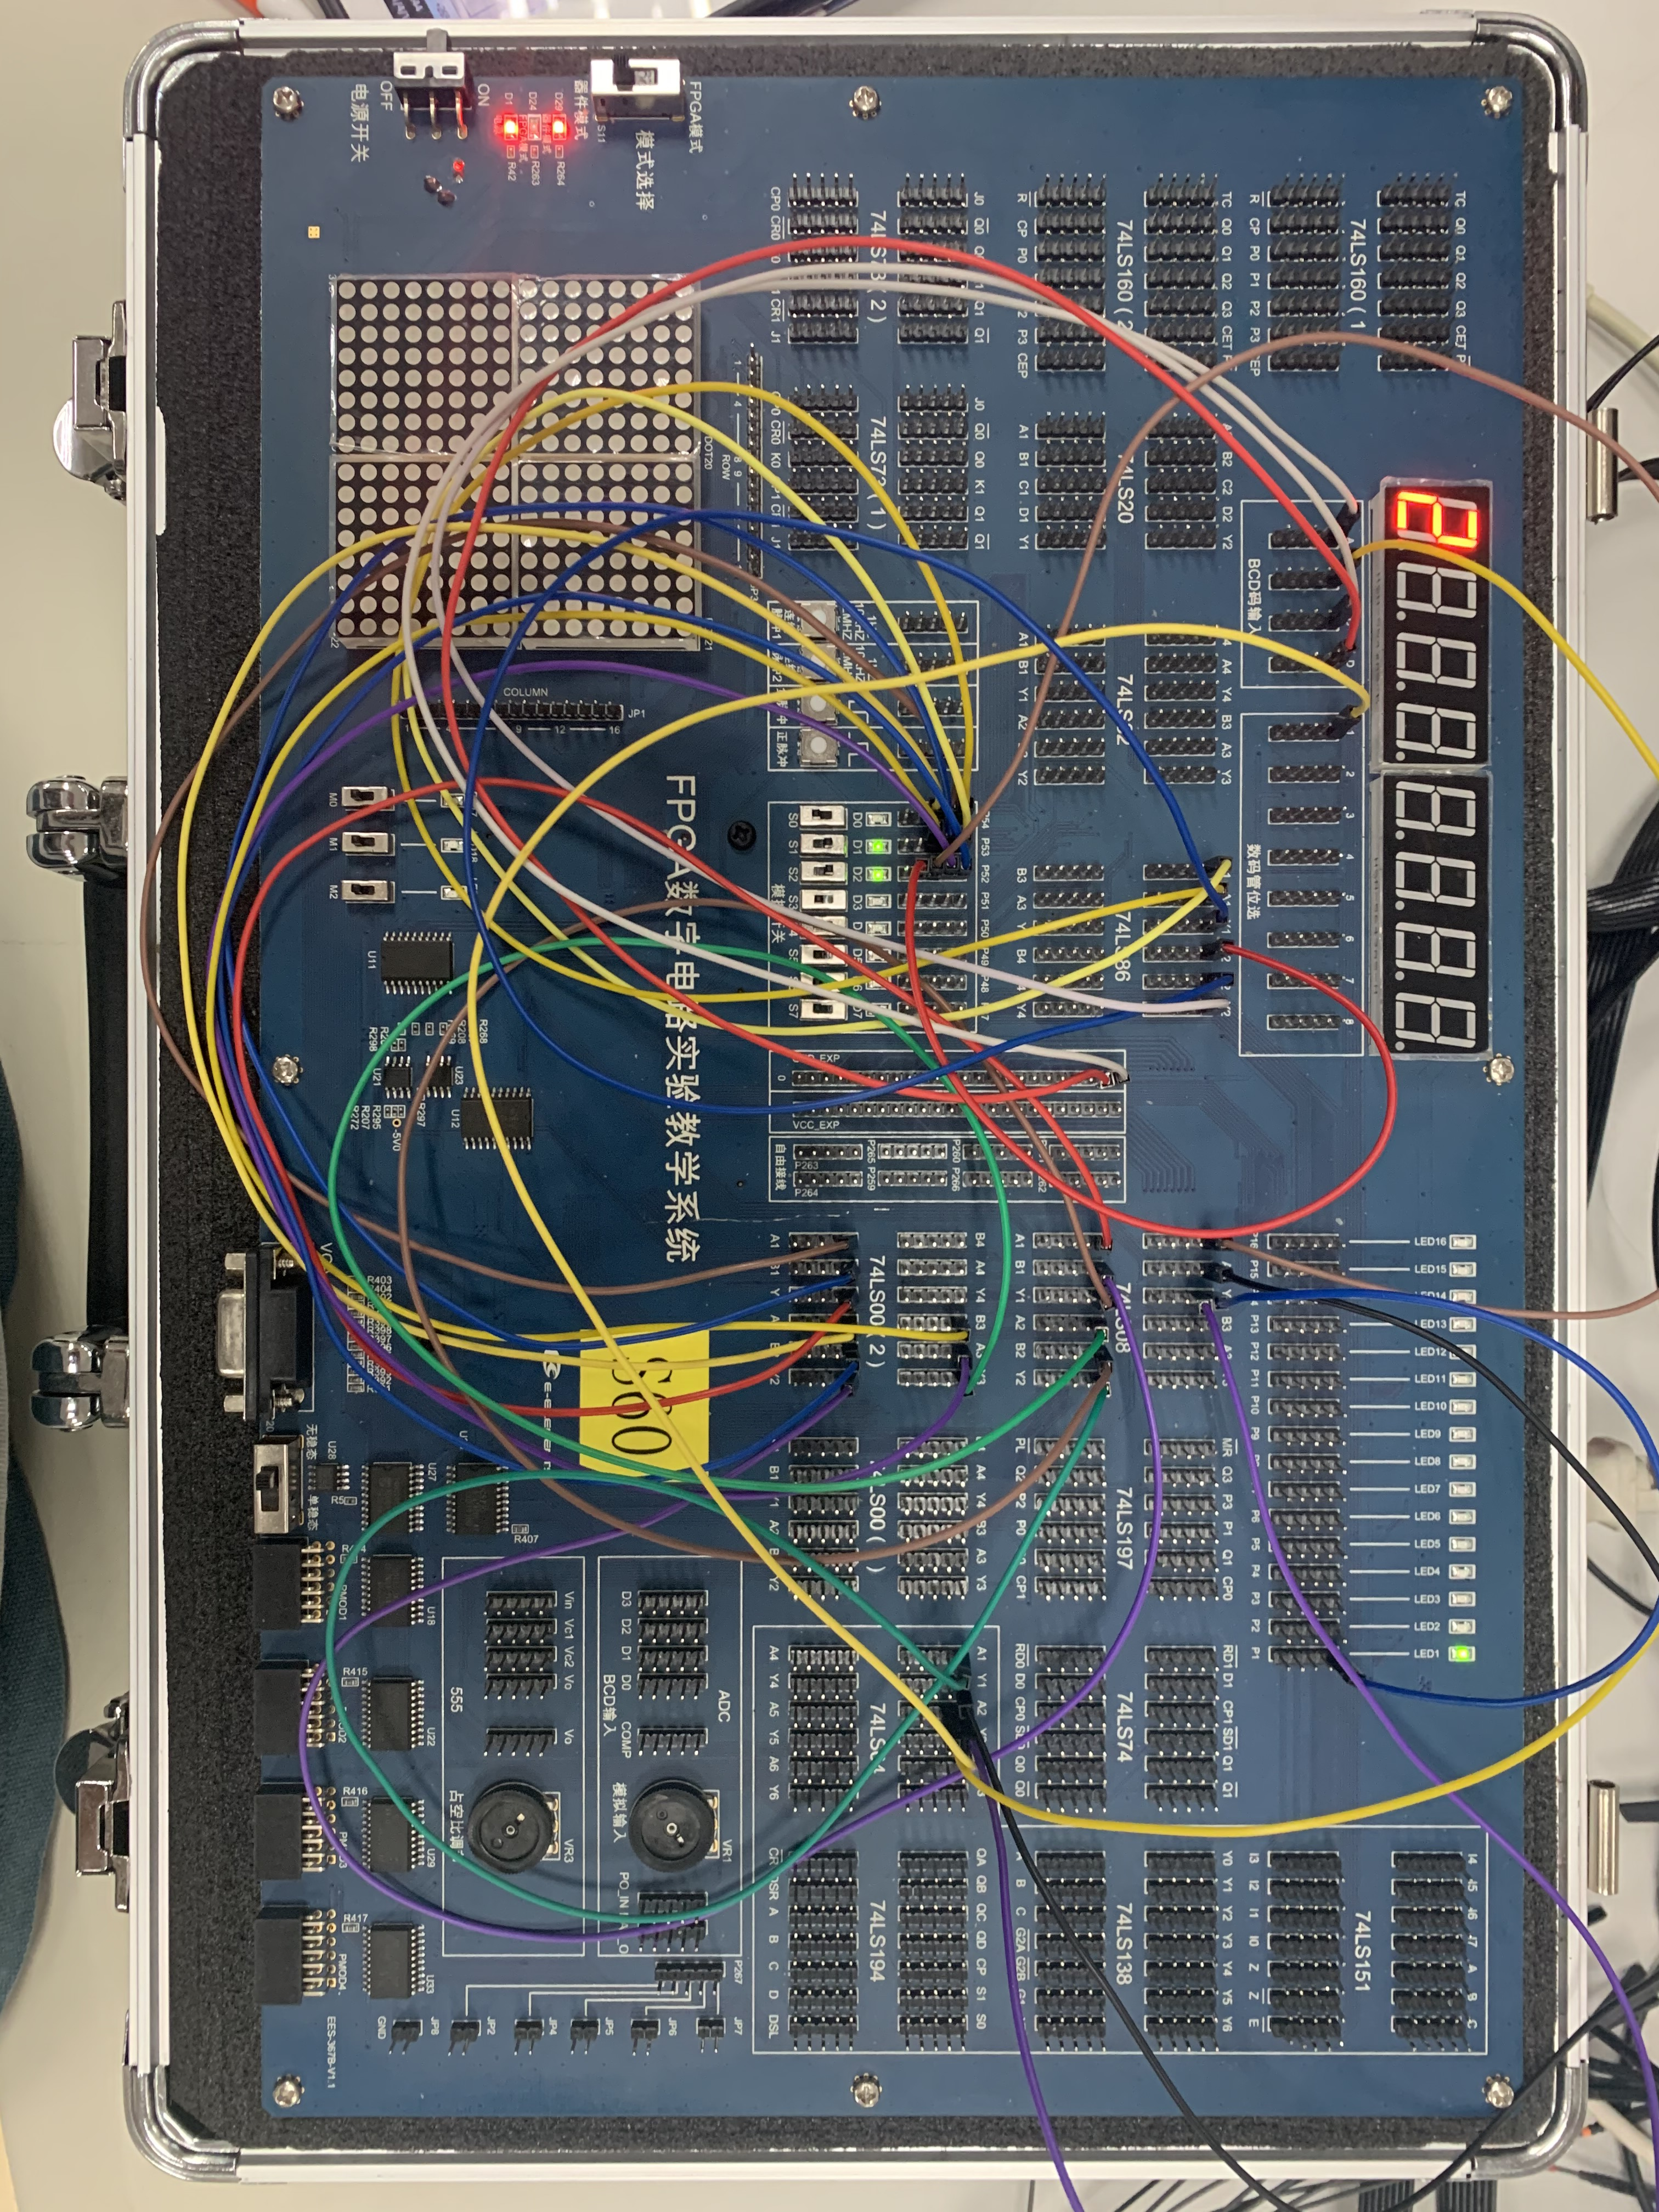
\includegraphics[width=0.8\textwidth]{箱110.png}
\end{figure}
\begin{figure}[H]
    \centering
    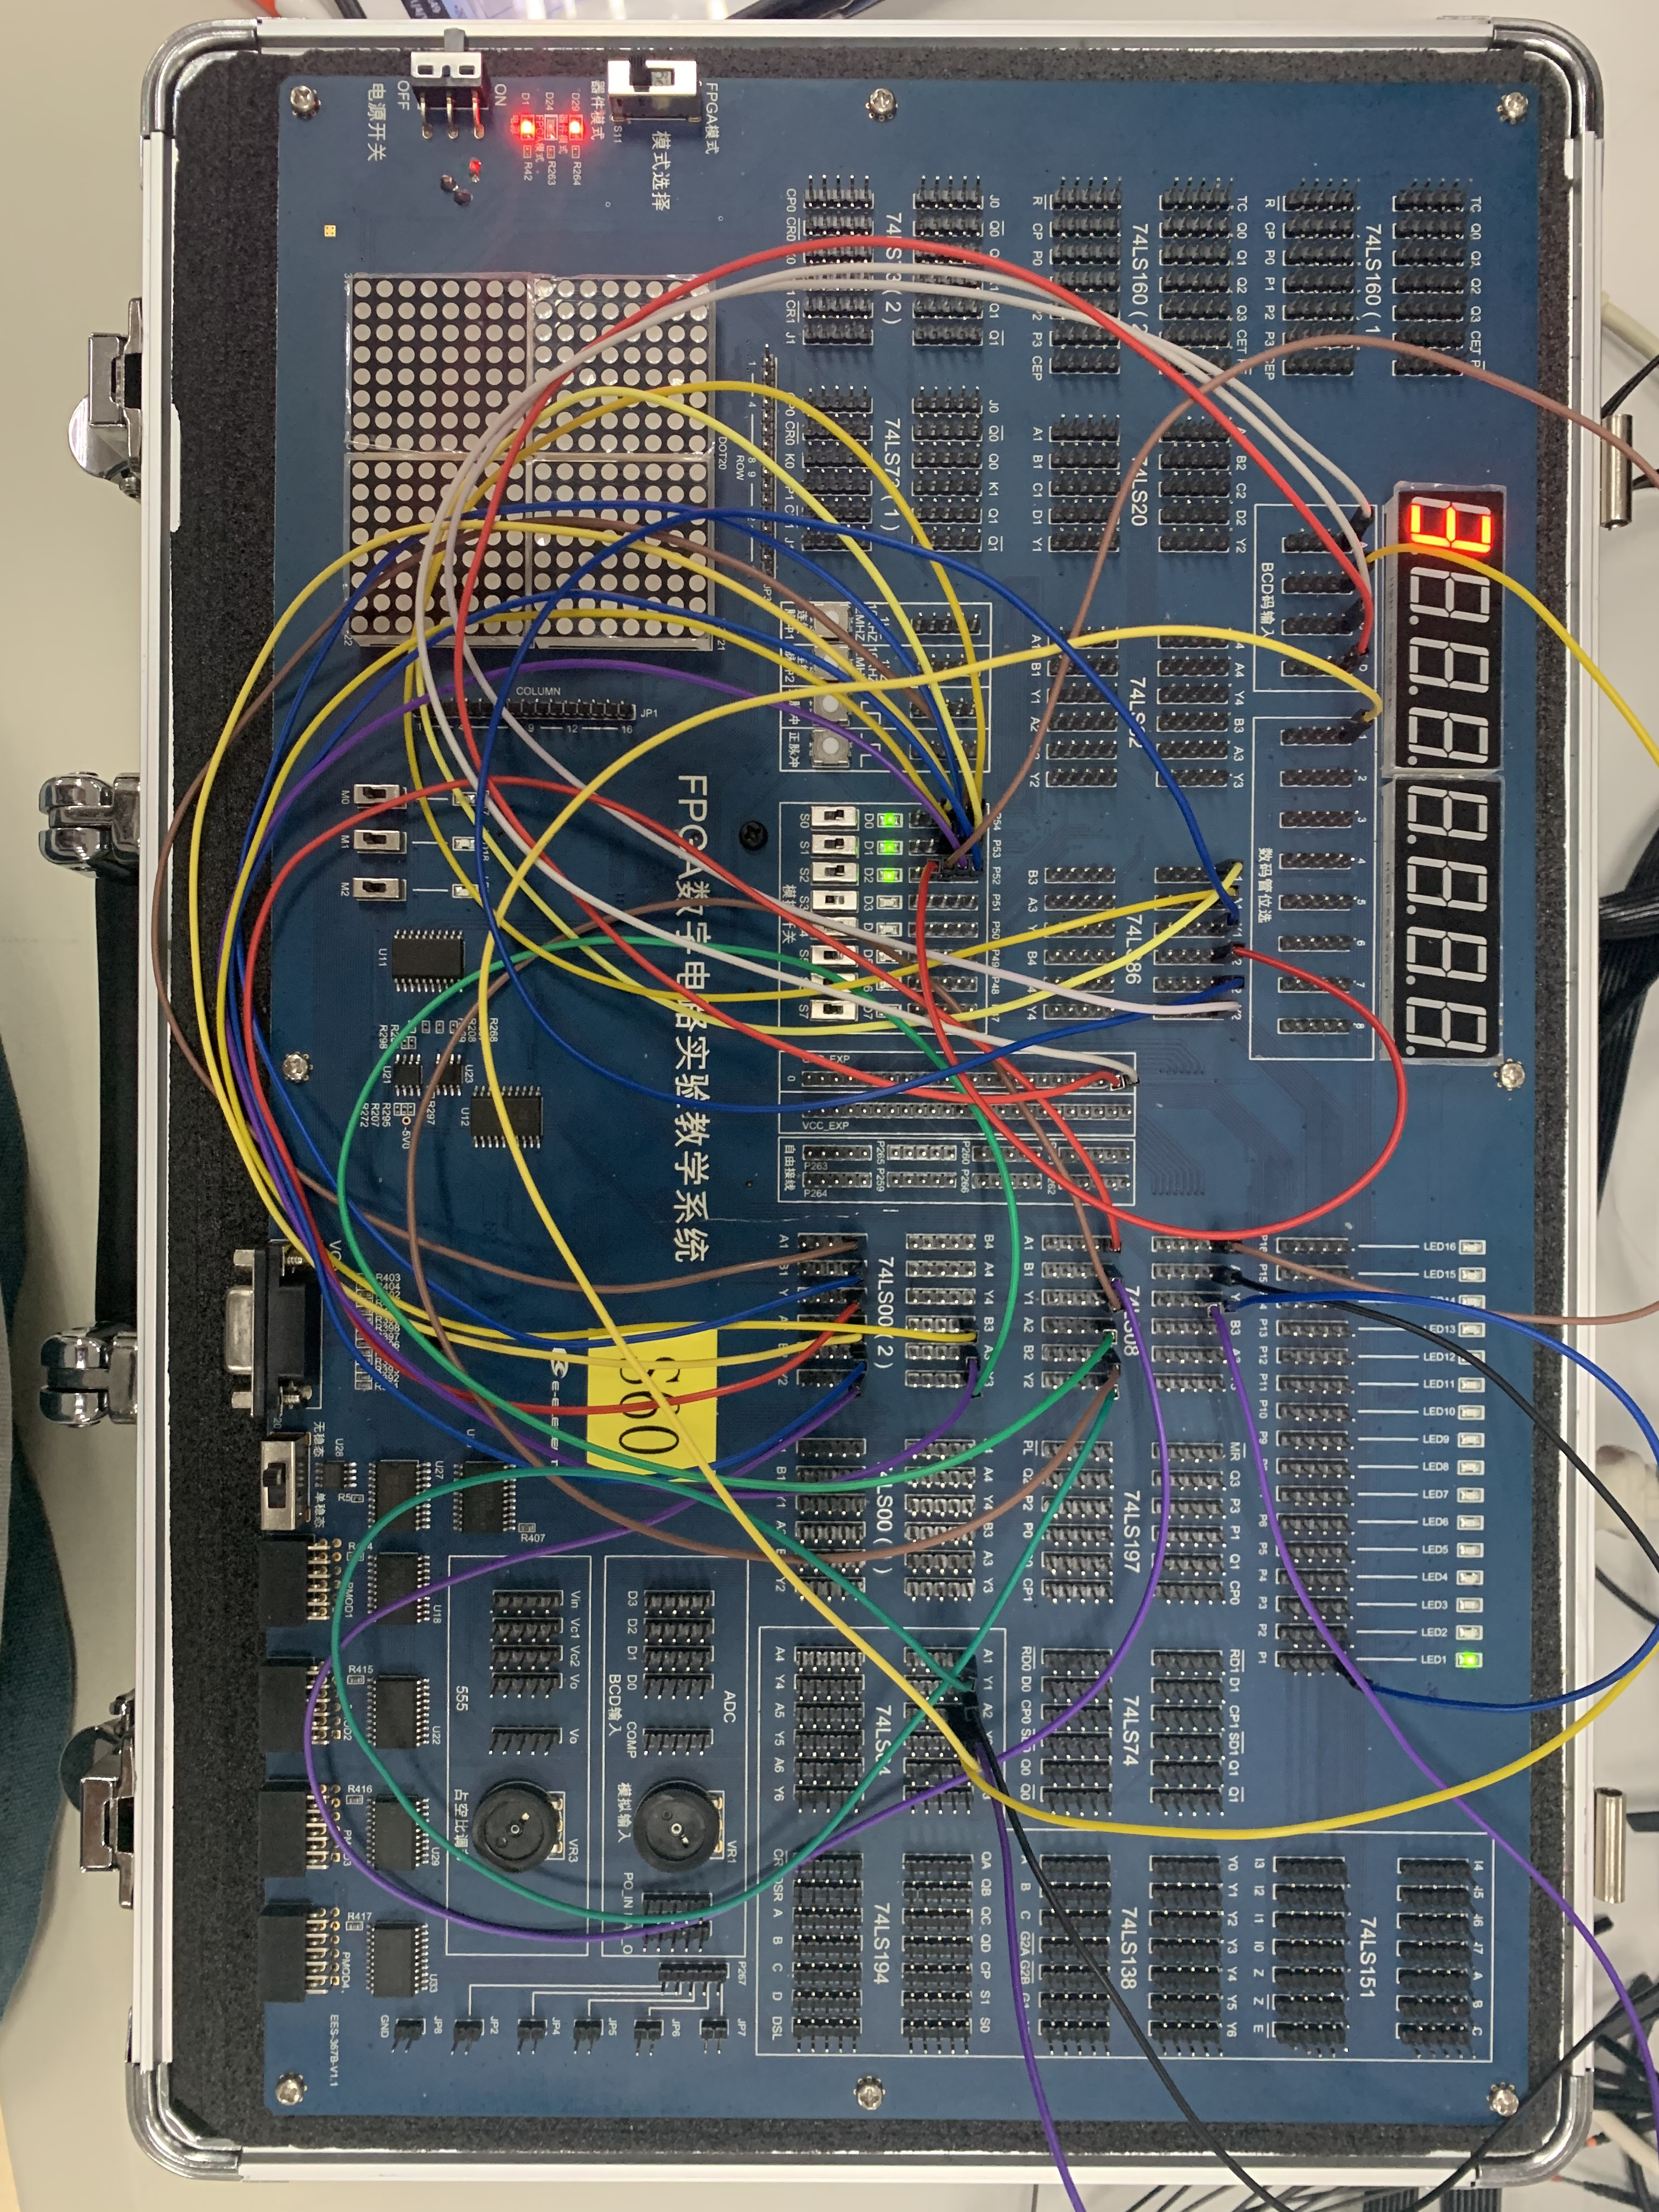
\includegraphics[width=0.8\textwidth]{箱111.png}
\end{figure}
\section{实验总结}
对加法器的了解更加深入。
%\clearpage
%\bibliography{E:/Papers/LiuLab}
%\bibliographystyle{apalike}
\end{document}
%%% Local Variables:
%%% mode: latex
%%% TeX-master: t
%%% End:
